Dieses Kapitel behandelt die elektronische Verarbeitung der BfArM-Daten. % unabhängig von einer konkreten technischen Implementierung. 

\section{Kode- und Umsteiger-Dateien}

Das BfArM stellt für jede neue ICD-10-GM- und OPS-Version Dateien für die Überleitung auf die Vorgänger-Version zum Download zur Verfügung, gebündelt jeweils in einer Zip-Datei: \cite[Downloads]{bfarmdl}.

Es handelt sich hierbei um CSV-formatierte Text-Dateien. CSV steht für "`Comma-Separated Values"' und ist ein sehr einfaches Format, um Daten zu strukturieren. Es wird ein Satzzeichen verwendet, um den restlichen Text in Spalten zu trennen -- laut dem Namen normalerweise ein Komma, aber für die BfArM-Dateien wurde Strichpunkt als Trennzeichen gewählt, wahrscheinlich weil die Klassentitel auch Kommata enthalten können. Weitere Informationen zum CSV Datei-Format finden sich hier: \cite[Seite 131f]{bonnefoy2024definitive}. 

Vom BfArM werden Kodes als Schlüsselnummern bezeichnet, wenn diese eindeutig sind und einzelne Überleitungen zwischen Kodes werden Umsteiger genannt.

\subsection{Kodes / Schlüsselnummern}

Hier beispielhaft die ersten sieben Zeilen der Kode-Datei von ICD-10-GM, Version 2024:

\codeBox{.79}{UNDEF;Undefined\newline
A00;Cholera\newline
A00.0;Cholera durch Vibrio cholerae O:1, Biovar cholerae\newline
A00.1;Cholera durch Vibrio cholerae O:1, Biovar eltor\newline
A00.9;Cholera, nicht näher bezeichnet\newline
A01;Typhus abdominalis und Paratyphus\newline
A01.0;Typhus abdominalis
}

Anmerkungen: 
\begin{itemize}
\item Ein Strichpunkt = zwei Spalten
\begin{enumerate}
\item Kode
\item Klassentitel
\end{enumerate}
\item Für OPS ist das Format der Kode-Datei identisch.
\item Mit Ausnahme des UNDEF-Eintrags in der ersten Zeile ist die Datei alphabetisch nach dem Kode sortiert. UNDEF ist kein ICD-10-GM- oder OPS-Kode, sondern wird für Umsteiger verwendet, um entfernte beziehungsweise neu hinzugefügte Kodes zu kennzeichnen.
\item Die Datei enthält nicht-endständige Kodes -- im Beispiel oben A00 und A01. Ein Kode ist endständig, wenn er keine Subkategorie hat. \cite[Kategorie und Kode in der ICD-10-GM]{bfarmicdkk}
\end{itemize}

\subsection{Umsteiger / Überleitungen}

Im Gegensatz zu den Kodes haben die Umsteiger für ICD-10-GM und OPS unterschiedliche Formate. Hier also zuerst zwei Ausschnitte aus der Umsteiger-Datei für ICD-10-GM, Version 2017 Überleitung auf Version 2016:

\codeBoxDouble{.27}{A00.0;A00.0;A;A\newline
A00.1;A00.1;A;A\newline
A00.9;A00.9;A;A\newline
A01.0;A01.0;A;A\newline
A01.1;A01.1;A;A}
{U06.0;UNDEF;A;\newline
UNDEF;Z99.0;;\newline
Z99.0;Z99.0;A;
}

Anmerkungen: 
\begin{itemize}
\item Drei Strichpunkte = vier Spalten
\begin{enumerate}
\item Alter Kode (2016)
\item Neuer Kode (2017)
\item Wenn A: automatisch überleitbar von 2016 auf 2017, sonst nicht
\item Wenn A: automatisch überleitbar von 2017 auf 2016, sonst nicht
\end{enumerate}
\item Der obere Abschnitt umfasst die fünf ersten Zeilen der Umsteiger-Datei. 
\item Der untere Abschnitt enthält beispielhaft zwei Umsteiger mit UNDEF. UNDEF als neuer Kode heißt der alte Kode wurde entfernt. UNDEF als alter Kode heißt der neue Kode wurde hinzugefügt. In diesem Beispiel wurde Z99.0 umbenannt. 
\item Die Datei ist alphabetisch nach dem alten Kode sortiert und falls dieser bei mehreren Einträgen identisch ist, anschließend nach dem neuen Kode.
\item Es sind nur endständige Kodes enthalten. 
\end{itemize}

Dazu im Vergleich ein einzelner Umsteiger aus dem OPS, Version 2024 Überleitung auf Version 2023:

\codeBox{.3}{1-100;N;1-100;N;A;A}

Die zusätzlichen Spalten jeweils nach den Kodes speziell für OPS sagen aus, ob Zusatzkennzeichen notwendig sind, siehe dazu auch: \cite[Kategorie und Kode im OPS]{bfarmopskk}.

\subsection{"`DRY"'-Prinzip}

"`Don't Repeat Yourself"' ist eines der Kardinalprinzipien in der Software-Entwicklung. Obwohl der Grundsatz, Wiederholungen zu vermeiden, wahrscheinlich schon in der Programmierung angewandt wird seit es diesen Beruf gibt, wurde "`DRY"' erstmals 1999 ausformuliert von \cite[Seite 79ff]{thomas2019pragmatic}. In der zwanzigjährigen Jubiläumsausgabe verdeutlichen die Autoren, dass es ihnen hierbei nicht nur um das Schreiben von Programmcode geht, sondern vielmehr um die Absichten hinter einem Prozess. Das heißt eine Änderung der Intention einer Software-Lösung sollte nicht mehrere Änderungen an mehreren Stellen nach sich ziehen. 

Bei der Integration der BfArM-Daten kann das "`DRY"'-Prinzip auf zwei Arten angewandt werden.

\begin{enumerate}
\item Bezogen auf Kodiersysteme: Alle Funktionen sollten unabhängig davon funktionieren, ob es sich um ICD-10-GM- oder OPS-Daten handelt. Auch die Aufnahme eines zusätzlichen Systems, beispielsweise ATC, sollte möglichst nur Anpassungen erfordern, die durch Abweichungen in der Integration der Daten dieses Systems notwendig sind. 
\item Bezogen auf Versionen: Der Prozess der Datenintegration sollte unabhängig von der Version gleich ablaufen und das gleiche Ergebnis liefern, bezogen auf die Datenstruktur. Jede Abweichung zwischen Versionen sollte nur eine möglichst einfach zu implementierende Modifikation des Gesamtprozesses darstellen. Konkret heißt das beim Hinzufügen einer neuen Version, dass an nur einer Stelle die Abweichungen von der Standardversion angegeben werden sollten und der Datenintegrationsprozess danach einmal angestoßen wird. Idealerweise ändert sich bei einer neuen Version nur die Versionsnummer und die Download-URL. 
\end{enumerate}

\subsection{Standardverfahren und Abweichungen}
\label{struktdateiversionen}

Im diesem Abschnitt werden alle Abweichungen der ICD-10-GM- und OPS-Versionen von der als Standard gewählten Version 2024 in Tabellen aufgeführt. Konkret gemeinst sind damit: Version, Download-URL, Pfad der Kode- und Umsteiger-Dateien, Sonstiges. Diese Informationen können dann dem Datenintegrationsprozess in einem strukturierten Dateiformat zur Verfügung gestellt werden. {\color{blue} §TODO: Verweis auf konkrete Implementation}

\newpara{Liste aller Versionen}

Im Anhang \ref{abweichungen-versionen} befinden sich Tabellen, die alle Abweichungen zwischen den Versionen für ICD-10-GM und OPS bezogen auf 2024 enthalten.

\newpara{Datei-Adressen und -Pfade}

Die Download-URL der Zip-Dateien setzt sich wie folgt zusammen:

\begingroup
\renewcommand{\arraystretch}{1.0}
\begin{tabular}{p{4cm}l}
\multicolumn{2}{l}{\texttt{https://multimedia.gsb.bund.de/BfArM/downloads/klassifikationen/} \ldots} \\
\& für ICD-10-GM: & \texttt{icd-10/ \ldots} \\
\& für OPS: & \texttt{ops/ \ldots} \\
\multicolumn{2}{l}{\& einen pro Version unterschiedlichen Teil, siehe URL-Eintrag in den Tabellen.} \\
\multicolumn{2}{l}{Die URL dient damit als "`Single Source of Truth"' \cite[Seite 257]{bonnefoy2024definitive}.} \\
\end{tabular}
\endgroup \\

Die Kode- und Umsteiger-Dateien sind in einem Verzeichnis enthalten:

\begingroup
\renewcommand{\arraystretch}{1.0}
\begin{tabular}{l}
\texttt{Klassifikationsdateien} \\
Wenn die Tabellen einen Verzeichnis-Eintrag enthalten, wird dieser vorangestellt. \\
Zum Beispiel für ICD-10-GM Version 2021: \\
\texttt{icd10gm2021syst-ueberl-20201111/Klassifikationsdateien} \\
\end{tabular}
\endgroup \\

Der Pfad der Kode-Datei lautet:

\begingroup
\renewcommand{\arraystretch}{1.0}
\begin{tabular}{p{4cm}l}
Verzeichnis & \ldots \\
\& für ICD-10-GM: & \texttt{icd10gm} \ldots \\
\& für OPS: & \texttt{ops} \ldots \\
\& die Version & \ldots\\
\& \texttt{syst.txt} \\
\multicolumn{2}{l}{Also zum Beispiel: \texttt{Klassifikationsdateien/icd10gm2024syst.txt}} \\
\multicolumn{2}{l}{Wenn die Tabellen einen Kodes-Eintrag enthalten, gilt dieser stattdessen.} \\
\end{tabular}
\endgroup \\

Die Umsteiger-Datei funktioniert ähnlich, nur dass der Dateiname normalerweise so ist:

\begingroup
\renewcommand{\arraystretch}{1.0}
\begin{tabular}{p{4cm}l}
für ICD-10-GM: & \texttt{icd10gm} \ldots\\
für OPS: & \texttt{ops} \ldots\\
\& Version & \ldots\\
\& \texttt{syst\_umsteiger\_} & \ldots\\
\& Vorgänger-Version & \ldots\\
\& \texttt{\_} & \ldots\\
\& Version & \ldots\\
\& \texttt{.txt} & Zum Beispiel: \texttt{ops2024syst\_umsteiger\_2023\_2024.txt}\\
\end{tabular}
\endgroup \\

\newpara{Sonstige Abweichungen}
\label{abweichungen}

\begin{itemize}
\item Vorab-Version\newline Diese Version hat noch keine Seite für die Kode-Suche. {\color{blue} §TODO: Verweis auf Kode-Suche (Frontend)}
\item Zip-Unterdatei\newline Die Zip-Datei der 2022 Versionen enthielt weitere Zip-Dateien. Vorher wurden alle Dateien zu einer Versionen nach Verwendungszweck nur in Unterverzeichnisse gegliedert, weswegen die gebündelte Zip-Datei insgesamt relativ groß wurde. Ab 2023 werden die Zip-Unterdateien separat zum Download angeboten.
\item ISO-8859-1\newline Vor 2009 waren Dateien in ISO-8859-1 kodiert, auch Latin-1 genannt, statt UTF-8. Mehr dazu unter Abschnitt \ref{latin1-encoding}.
\item Punkt-Strich-Notation, Kreuz-Stern-System \newline Die Kodes älterer ICD-10-GM Versionen hatten Sonderzeichen gemäß \cite{bfarmicdkk}.
\item 6-Spalten-Umsteiger \newline Umsteiger älterer ICD-10-GM Versionen enthielten Informationen zur Mehrfachkodierung. 
\item Nicht endständige Umsteiger\newline Im Gegensatz zu allen anderen Überleitungen sind die Umsteiger-Einträge für ICD-10-GM 2.0 auf 1.3. auch für nicht-endständige Kodes enthalten. 
\item None statt UNDEF\newline Von OPS Version 2009 bis 2004 wurde statt UNDEF der Bezeichner "`None"' verwendet. 
\item KOMBI-Kode\newline OPS Versionen 2.1 und 2.0 enthalten in der Kodes-Datei einen zusätzlichen Eintrag: KOMBI, "`Kombinationsschlüsselnummer erforderlich"'. 
\item 6-Spalten-Umsteiger (altes Format), 5-Spalten-Umsteiger, 4-Spalten-Umsteiger\newline Die Umsteiger der OPS-Versionen von 2009 bis 2005 waren anders formatiert, weil 2005 die Informationen bezüglich Zusatzkennzeichen hinzukamen und bis 2009 die Spalten unterschiedlich angeordnet waren als in allen neueren OPS Versionen. 
\item 6-Spalten-Umsteiger (ursprüngliches Format)\newline Die Umsteiger für OPS Version 2.1 enthielen zusätzliche Spalten wegen Mehrfachverschlüsselung wie die älteren ICD-10-GM Versionen. 
\item 3-Spalten-Umsteiger\newline OPS Version 2.0 zeigte mit nur einer Spalte an, ob automatische Überleitungen möglich sind. 
\item Keine Überleitung\newline Aus der ältesten Version, die Überleitungen enthält, wird zusätzlich die Kodes-Datei für die Vorgänger-Versionen verarbeitet.
\end{itemize}

\section{Datenintegrationsprozess}

Wie erwähnt durchlaufen alle Daten unabhängig von Version und Kodiersystem den gleichen Integrationsprozess. Dieser orientiert sich an dem klassischen "`Extract-Transform-Load"' Modell, siehe \cite[Seite 247ff]{bonnefoy2024definitive}.

\begin{enumerate}
\item \emph{Extract:} Die Daten werden in einem bestimmten Format aus einem Quell-System extrahiert. 
\item \emph{Transform:} In einem oder mehreren Prozessen werden die Daten in ein standardisiertes Format transformiert, was zum Beispiel Bereinigung, Validierung und Imputation beinhalten kann.
\item \emph{Insert:} Die Daten werden in ein Ziel-System integriert, um dort von weiteren Applikationen verwendet zu werden. 
\end{enumerate}

%\vspace{10pt}

\begin{figure}[H]
    \centering
    \setlength{\fboxsep}{.02\linewidth}\color{black!20}\fbox{
    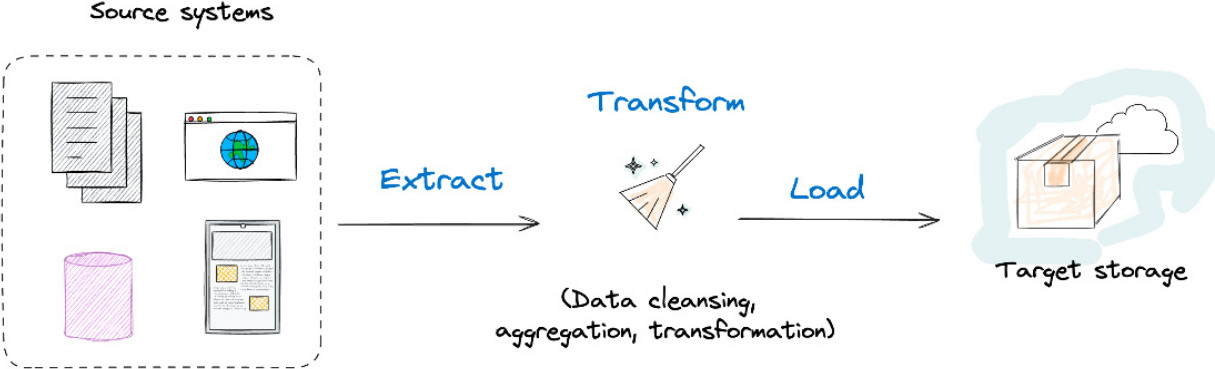
\includegraphics[width=.96\linewidth]{../img/etl.jpg}}
    \vspace{-10pt}
    \normalcolor\caption{ETL-Modell nach \cite[Seite 63]{bonnefoy2024definitive}}
\end{figure}

Für die BfArM-Daten sieht der Integrationsprozess konkret so aus:

\begin{enumerate}
\item \emph{Download:} Die Zip-Dateien werden heruntergeladen. Alternativ kann geprüft werden, ob die Dateien schon lokal vorhanden sind mit einem bestimmten Pfad, der sich nach Kodiersystem und Versionsnummer immer gleich zusammensetzt, zum Beispiel: \texttt{files/icd10gm2024.zip}. Die Download-Funktion sollte die Zip-Dateien ebenfalls unter diesem Pfad abspeichern, falls so gewünscht.
\item \emph{Unzip:} Die Kodes- und Umsteiger-Dateien werden aus der Zip-Datei extrahiert. Normalerweise muss dafür nicht das ganze Archiv in temporäre Dateien entpackt werden -- außer eventuell bei den Versionen 2022, weil das Extrahieren verschachtelter Zip-Dateien eher ein Nischenfall ist und nicht unbedingt standardmäßig von Programmiersprachen oder Bibliotheken unterstützt wird. 
\item \emph{Convert Encoding:}\label{latin1-encoding} Die in ISO-8859-1 kodierten Kodes-Dateien müssen in UTF-8 umgewandelt werden. In \cite{charencoding} werden die beiden Zeichenkodierungen genauer erklärt, aber für die BfArM-Daten ist eigentlich nur relevant, dass Umlaute mit unterschiedlichen Werten kodiert sind. Also würde das Einlesen eines in ISO-8859-1 kodierten Umlauts als UTF-8 ein anderes Zeichen als Resultat ergeben. Die Umsteiger-Dateien sind davon nicht betroffen, weil in diesen keine Umlaute enthalten sind. 
\item \emph{Parse CSV:} Ein Parser wandelt eine Datei in eine Datenstruktur um; für CSV sollte jede Programmiersprache so eine Funktion standardmäßig zur Verfügung stellen. Für die BfArM-Dateien ist das Ergebnis ein zweidimensionales Array mit zwei Spalten für die Kodes, beziehungsweise drei bis sechs Spalten für die Umsteiger je nach Kodiersystem und Version. 
\item \emph{Process Data:} Aufgrund der oben erwähnten Abweichungen ist die Vorverarbeitung der Daten der komplexeste Schritt und wird im nächsten Abschnitt genauer erklärt. Außerdem müssen nicht alle Daten gespeichert werden. Vor allem in Bezug auf die Zip-Dateien ergibt das eine Reduktion der Datenmenge um etwa einen Faktor von zehn. 
\item \emph{Insert:} Die bearbeiteten Daten werden für die Verwendung durch Applikationen gespeichert. Zum Beispiel für eine relationale Datenbank werden pro Dateityp, Kodiersystem und Version eine Tabelle angelegt und die Daten in diese geschrieben. Konkret für SQL müssen außerdem die Hochkommata in den Codes-Dateien beachtet werden. 
\end{enumerate}

\begin{figure}[H]
    \centering\large
    \resizebox{.9\textwidth}{!}{% Graphic for TeX using PGF
% Title: /home/simon/jacuke_ma/tex/dia/data-integration.dia
% Creator: Dia v0.97+git
% CreationDate: Wed Sep 11 07:50:56 2024
% For: simon
% \usepackage{tikz}
% The following commands are not supported in PSTricks at present
% We define them conditionally, so when they are implemented,
% this pgf file will use them.
\ifx\du\undefined
  \newlength{\du}
\fi
\setlength{\du}{15\unitlength}
\begin{tikzpicture}[even odd rule]
\pgftransformxscale{1.000000}
\pgftransformyscale{-1.000000}
\definecolor{dialinecolor}{rgb}{0.000000, 0.000000, 0.000000}
\pgfsetstrokecolor{dialinecolor}
\pgfsetstrokeopacity{1.000000}
\definecolor{diafillcolor}{rgb}{1.000000, 1.000000, 1.000000}
\pgfsetfillcolor{diafillcolor}
\pgfsetfillopacity{1.000000}
\pgfsetlinewidth{0.100000\du}
\pgfsetdash{}{0pt}
\pgfsetmiterjoin
\pgfsetbuttcap
{\pgfsetcornersarced{\pgfpoint{0.000000\du}{0.000000\du}}\definecolor{diafillcolor}{rgb}{1.000000, 1.000000, 1.000000}
\pgfsetfillcolor{diafillcolor}
\pgfsetfillopacity{0.396078}
\fill (19.000000\du,-6.000000\du)--(19.000000\du,22.000000\du)--(52.000000\du,22.000000\du)--(52.000000\du,-6.000000\du)--cycle;
}{\pgfsetcornersarced{\pgfpoint{0.000000\du}{0.000000\du}}\definecolor{dialinecolor}{rgb}{1.000000, 1.000000, 1.000000}
\pgfsetstrokecolor{dialinecolor}
\pgfsetstrokeopacity{1.000000}
\draw (19.000000\du,-6.000000\du)--(19.000000\du,22.000000\du)--(52.000000\du,22.000000\du)--(52.000000\du,-6.000000\du)--cycle;
}\pgfsetlinewidth{0.100000\du}
\pgfsetdash{}{0pt}
\pgfsetbuttcap
\pgfsetmiterjoin
\pgfsetlinewidth{0.001000\du}
\pgfsetbuttcap
\pgfsetmiterjoin
\pgfsetdash{}{0pt}
\definecolor{diafillcolor}{rgb}{0.717647, 0.717647, 0.615686}
\pgfsetfillcolor{diafillcolor}
\pgfsetfillopacity{1.000000}
\pgfpathmoveto{\pgfpoint{21.000000\du}{-3.393141\du}}
\pgfpathlineto{\pgfpoint{21.000000\du}{4.150583\du}}
\pgfpathlineto{\pgfpoint{25.458746\du}{4.150583\du}}
\pgfpathlineto{\pgfpoint{25.458746\du}{-3.393141\du}}
\pgfpathlineto{\pgfpoint{21.000000\du}{-3.393141\du}}
\pgfpathclose
\pgfusepath{fill}
\pgfsetbuttcap
\pgfsetmiterjoin
\pgfsetdash{}{0pt}
\definecolor{dialinecolor}{rgb}{0.286275, 0.286275, 0.211765}
\pgfsetstrokecolor{dialinecolor}
\pgfsetstrokeopacity{1.000000}
\pgfpathmoveto{\pgfpoint{21.000000\du}{-3.393141\du}}
\pgfpathlineto{\pgfpoint{21.000000\du}{4.150583\du}}
\pgfpathlineto{\pgfpoint{25.458746\du}{4.150583\du}}
\pgfpathlineto{\pgfpoint{25.458746\du}{-3.393141\du}}
\pgfpathlineto{\pgfpoint{21.000000\du}{-3.393141\du}}
\pgfusepath{stroke}
\pgfsetbuttcap
\pgfsetmiterjoin
\pgfsetdash{}{0pt}
\definecolor{diafillcolor}{rgb}{0.788235, 0.788235, 0.713726}
\pgfsetfillcolor{diafillcolor}
\pgfsetfillopacity{1.000000}
\pgfpathmoveto{\pgfpoint{21.000000\du}{-3.393141\du}}
\pgfpathlineto{\pgfpoint{21.604191\du}{-4.000000\du}}
\pgfpathlineto{\pgfpoint{26.061604\du}{-4.000000\du}}
\pgfpathlineto{\pgfpoint{25.458746\du}{-3.393141\du}}
\pgfpathlineto{\pgfpoint{21.000000\du}{-3.393141\du}}
\pgfpathclose
\pgfusepath{fill}
\pgfsetbuttcap
\pgfsetmiterjoin
\pgfsetdash{}{0pt}
\definecolor{dialinecolor}{rgb}{0.286275, 0.286275, 0.211765}
\pgfsetstrokecolor{dialinecolor}
\pgfsetstrokeopacity{1.000000}
\pgfpathmoveto{\pgfpoint{21.000000\du}{-3.393141\du}}
\pgfpathlineto{\pgfpoint{21.604191\du}{-4.000000\du}}
\pgfpathlineto{\pgfpoint{26.032261\du}{-4.000000\du}}
\pgfusepath{stroke}
\pgfsetbuttcap
\pgfsetmiterjoin
\pgfsetdash{}{0pt}
\definecolor{dialinecolor}{rgb}{0.286275, 0.286275, 0.211765}
\pgfsetstrokecolor{dialinecolor}
\pgfsetstrokeopacity{1.000000}
\pgfpathmoveto{\pgfpoint{26.032261\du}{-3.969324\du}}
\pgfpathlineto{\pgfpoint{25.458746\du}{-3.393141\du}}
\pgfpathlineto{\pgfpoint{21.000000\du}{-3.393141\du}}
\pgfusepath{stroke}
\pgfsetbuttcap
\pgfsetmiterjoin
\pgfsetdash{}{0pt}
\definecolor{diafillcolor}{rgb}{0.788235, 0.788235, 0.713726}
\pgfsetfillcolor{diafillcolor}
\pgfsetfillopacity{1.000000}
\pgfpathmoveto{\pgfpoint{21.274754\du}{-2.954335\du}}
\pgfpathlineto{\pgfpoint{23.311399\du}{-2.954335\du}}
\pgfpathlineto{\pgfpoint{23.311399\du}{-1.964688\du}}
\pgfpathlineto{\pgfpoint{21.274754\du}{-1.964688\du}}
\pgfpathlineto{\pgfpoint{21.274754\du}{-2.954335\du}}
\pgfpathclose
\pgfusepath{fill}
\pgfsetbuttcap
\pgfsetmiterjoin
\pgfsetdash{}{0pt}
\definecolor{dialinecolor}{rgb}{0.384314, 0.384314, 0.282353}
\pgfsetstrokecolor{dialinecolor}
\pgfsetstrokeopacity{1.000000}
\pgfpathmoveto{\pgfpoint{21.274754\du}{-2.954335\du}}
\pgfpathlineto{\pgfpoint{23.310065\du}{-2.954335\du}}
\pgfpathlineto{\pgfpoint{23.310065\du}{-1.966022\du}}
\pgfpathlineto{\pgfpoint{21.274754\du}{-1.966022\du}}
\pgfpathlineto{\pgfpoint{21.274754\du}{-2.954335\du}}
\pgfusepath{stroke}
\pgfsetlinewidth{0.030000\du}
\pgfsetbuttcap
\pgfsetmiterjoin
\pgfsetdash{}{0pt}
\definecolor{dialinecolor}{rgb}{0.925490, 0.925490, 0.905882}
\pgfsetstrokecolor{dialinecolor}
\pgfsetstrokeopacity{1.000000}
\pgfpathmoveto{\pgfpoint{21.549507\du}{-2.458178\du}}
\pgfpathlineto{\pgfpoint{22.977960\du}{-2.458178\du}}
\pgfusepath{stroke}
\pgfsetlinewidth{0.001000\du}
\pgfsetbuttcap
\pgfsetmiterjoin
\pgfsetdash{}{0pt}
\definecolor{diafillcolor}{rgb}{0.478431, 0.478431, 0.352941}
\pgfsetfillcolor{diafillcolor}
\pgfsetfillopacity{1.000000}
\pgfpathmoveto{\pgfpoint{25.458746\du}{4.150583\du}}
\pgfpathlineto{\pgfpoint{26.061604\du}{3.542390\du}}
\pgfpathlineto{\pgfpoint{26.061604\du}{-4.000000\du}}
\pgfpathlineto{\pgfpoint{25.458746\du}{-3.393141\du}}
\pgfpathlineto{\pgfpoint{25.458746\du}{4.150583\du}}
\pgfpathclose
\pgfusepath{fill}
\pgfsetbuttcap
\pgfsetmiterjoin
\pgfsetdash{}{0pt}
\definecolor{dialinecolor}{rgb}{0.286275, 0.286275, 0.211765}
\pgfsetstrokecolor{dialinecolor}
\pgfsetstrokeopacity{1.000000}
\pgfpathmoveto{\pgfpoint{25.458746\du}{4.150583\du}}
\pgfpathlineto{\pgfpoint{26.032261\du}{3.573067\du}}
\pgfusepath{stroke}
\pgfsetbuttcap
\pgfsetmiterjoin
\pgfsetdash{}{0pt}
\definecolor{dialinecolor}{rgb}{0.286275, 0.286275, 0.211765}
\pgfsetstrokecolor{dialinecolor}
\pgfsetstrokeopacity{1.000000}
\pgfpathmoveto{\pgfpoint{26.032261\du}{-3.969324\du}}
\pgfpathlineto{\pgfpoint{25.458746\du}{-3.393141\du}}
\pgfpathlineto{\pgfpoint{25.458746\du}{4.150583\du}}
\pgfusepath{stroke}
\pgfsetlinewidth{0.030000\du}
\pgfsetbuttcap
\pgfsetmiterjoin
\pgfsetdash{}{0pt}
\definecolor{dialinecolor}{rgb}{0.925490, 0.925490, 0.905882}
\pgfsetstrokecolor{dialinecolor}
\pgfsetstrokeopacity{1.000000}
\pgfpathmoveto{\pgfpoint{21.056018\du}{3.653092\du}}
\pgfpathlineto{\pgfpoint{25.457413\du}{3.653092\du}}
\pgfusepath{stroke}
\pgfsetbuttcap
\pgfsetmiterjoin
\pgfsetdash{}{0pt}
\definecolor{dialinecolor}{rgb}{0.000000, 0.000000, 0.000000}
\pgfsetstrokecolor{dialinecolor}
\pgfsetstrokeopacity{1.000000}
\pgfpathmoveto{\pgfpoint{21.056018\du}{-0.365515\du}}
\pgfpathlineto{\pgfpoint{25.457413\du}{-0.365515\du}}
\pgfusepath{stroke}
\pgfsetbuttcap
\pgfsetmiterjoin
\pgfsetdash{}{0pt}
\definecolor{dialinecolor}{rgb}{0.286275, 0.286275, 0.211765}
\pgfsetstrokecolor{dialinecolor}
\pgfsetstrokeopacity{1.000000}
\pgfpathmoveto{\pgfpoint{21.000000\du}{3.598408\du}}
\pgfpathlineto{\pgfpoint{25.453411\du}{3.598408\du}}
\pgfusepath{stroke}
\pgfsetbuttcap
\pgfsetmiterjoin
\pgfsetdash{}{0pt}
\definecolor{dialinecolor}{rgb}{0.000000, 0.000000, 0.000000}
\pgfsetstrokecolor{dialinecolor}
\pgfsetstrokeopacity{1.000000}
\pgfpathmoveto{\pgfpoint{21.000000\du}{-0.421533\du}}
\pgfpathlineto{\pgfpoint{25.453411\du}{-0.421533\du}}
\pgfusepath{stroke}
\pgfsetlinewidth{0.001000\du}
\pgfsetbuttcap
\pgfsetmiterjoin
\pgfsetdash{}{0pt}
\definecolor{dialinecolor}{rgb}{0.925490, 0.925490, 0.905882}
\pgfsetstrokecolor{dialinecolor}
\pgfsetstrokeopacity{1.000000}
\pgfpathmoveto{\pgfpoint{21.274754\du}{-2.018039\du}}
\pgfpathlineto{\pgfpoint{21.274754\du}{-2.954335\du}}
\pgfpathlineto{\pgfpoint{23.255381\du}{-2.954335\du}}
\pgfusepath{stroke}
\pgfsetlinewidth{0.100000\du}
\pgfsetdash{}{0pt}
\pgfsetbuttcap
\pgfsetmiterjoin
\pgfsetlinewidth{0.001000\du}
\pgfsetbuttcap
\pgfsetmiterjoin
\pgfsetdash{}{0pt}
\definecolor{diafillcolor}{rgb}{0.647059, 0.647059, 0.521569}
\pgfsetfillcolor{diafillcolor}
\pgfsetfillopacity{1.000000}
\pgfpathmoveto{\pgfpoint{51.124567\du}{17.183102\du}}
\pgfpathlineto{\pgfpoint{51.119703\du}{17.120845\du}}
\pgfpathlineto{\pgfpoint{51.106085\du}{17.059561\du}}
\pgfpathlineto{\pgfpoint{51.082738\du}{16.998276\du}}
\pgfpathlineto{\pgfpoint{51.050637\du}{16.937964\du}}
\pgfpathlineto{\pgfpoint{51.010753\du}{16.877653\du}}
\pgfpathlineto{\pgfpoint{50.961142\du}{16.818314\du}}
\pgfpathlineto{\pgfpoint{50.902776\du}{16.759947\du}}
\pgfpathlineto{\pgfpoint{50.835655\du}{16.702554\du}}
\pgfpathlineto{\pgfpoint{50.759778\du}{16.646133\du}}
\pgfpathlineto{\pgfpoint{50.676120\du}{16.592631\du}}
\pgfpathlineto{\pgfpoint{50.584680\du}{16.539129\du}}
\pgfpathlineto{\pgfpoint{50.486430\du}{16.486599\du}}
\pgfpathlineto{\pgfpoint{50.378453\du}{16.436988\du}}
\pgfpathlineto{\pgfpoint{50.264639\du}{16.389322\du}}
\pgfpathlineto{\pgfpoint{50.144015\du}{16.343602\du}}
\pgfpathlineto{\pgfpoint{50.015609\du}{16.299827\du}}
\pgfpathlineto{\pgfpoint{49.882340\du}{16.258971\du}}
\pgfpathlineto{\pgfpoint{49.742261\du}{16.220060\du}}
\pgfpathlineto{\pgfpoint{49.597318\du}{16.184068\du}}
\pgfpathlineto{\pgfpoint{49.445566\du}{16.150021\du}}
\pgfpathlineto{\pgfpoint{49.290896\du}{16.117919\du}}
\pgfpathlineto{\pgfpoint{49.130389\du}{16.089709\du}}
\pgfpathlineto{\pgfpoint{48.965991\du}{16.062471\du}}
\pgfpathlineto{\pgfpoint{48.799647\du}{16.040098\du}}
\pgfpathlineto{\pgfpoint{48.628439\du}{16.020642\du}}
\pgfpathlineto{\pgfpoint{48.454314\du}{16.004105\du}}
\pgfpathlineto{\pgfpoint{48.279215\du}{15.989514\du}}
\pgfpathlineto{\pgfpoint{48.101198\du}{15.979786\du}}
\pgfpathlineto{\pgfpoint{47.922208\du}{15.971031\du}}
\pgfpathlineto{\pgfpoint{47.742246\du}{15.965194\du}}
\pgfpathlineto{\pgfpoint{47.562284\du}{15.965194\du}}
\pgfpathlineto{\pgfpoint{47.562284\du}{15.965194\du}}
\pgfpathlineto{\pgfpoint{47.381348\du}{15.965194\du}}
\pgfpathlineto{\pgfpoint{47.201386\du}{15.971031\du}}
\pgfpathlineto{\pgfpoint{47.022396\du}{15.979786\du}}
\pgfpathlineto{\pgfpoint{46.844379\du}{15.989514\du}}
\pgfpathlineto{\pgfpoint{46.669281\du}{16.004105\du}}
\pgfpathlineto{\pgfpoint{46.495155\du}{16.020642\du}}
\pgfpathlineto{\pgfpoint{46.324920\du}{16.040098\du}}
\pgfpathlineto{\pgfpoint{46.157604\du}{16.062471\du}}
\pgfpathlineto{\pgfpoint{45.993206\du}{16.089709\du}}
\pgfpathlineto{\pgfpoint{45.832699\du}{16.117919\du}}
\pgfpathlineto{\pgfpoint{45.678028\du}{16.150021\du}}
\pgfpathlineto{\pgfpoint{45.527249\du}{16.184068\du}}
\pgfpathlineto{\pgfpoint{45.382306\du}{16.220060\du}}
\pgfpathlineto{\pgfpoint{45.242227\du}{16.258971\du}}
\pgfpathlineto{\pgfpoint{45.107985\du}{16.299827\du}}
\pgfpathlineto{\pgfpoint{44.979579\du}{16.343602\du}}
\pgfpathlineto{\pgfpoint{44.859929\du}{16.389322\du}}
\pgfpathlineto{\pgfpoint{44.745142\du}{16.436988\du}}
\pgfpathlineto{\pgfpoint{44.638137\du}{16.486599\du}}
\pgfpathlineto{\pgfpoint{44.538915\du}{16.539129\du}}
\pgfpathlineto{\pgfpoint{44.447474\du}{16.592631\du}}
\pgfpathlineto{\pgfpoint{44.363816\du}{16.646133\du}}
\pgfpathlineto{\pgfpoint{44.287940\du}{16.702554\du}}
\pgfpathlineto{\pgfpoint{44.220819\du}{16.759947\du}}
\pgfpathlineto{\pgfpoint{44.162453\du}{16.818314\du}}
\pgfpathlineto{\pgfpoint{44.112841\du}{16.877653\du}}
\pgfpathlineto{\pgfpoint{44.072958\du}{16.937964\du}}
\pgfpathlineto{\pgfpoint{44.040856\du}{16.998276\du}}
\pgfpathlineto{\pgfpoint{44.017510\du}{17.059561\du}}
\pgfpathlineto{\pgfpoint{44.004864\du}{17.120845\du}}
\pgfpathlineto{\pgfpoint{44.000000\du}{17.183102\du}}
\pgfpathlineto{\pgfpoint{44.000000\du}{17.183102\du}}
\pgfpathlineto{\pgfpoint{44.004864\du}{17.245360\du}}
\pgfpathlineto{\pgfpoint{44.017510\du}{17.305671\du}}
\pgfpathlineto{\pgfpoint{44.040856\du}{17.367929\du}}
\pgfpathlineto{\pgfpoint{44.072958\du}{17.428240\du}}
\pgfpathlineto{\pgfpoint{44.112841\du}{17.488552\du}}
\pgfpathlineto{\pgfpoint{44.162453\du}{17.547891\du}}
\pgfpathlineto{\pgfpoint{44.220819\du}{17.606257\du}}
\pgfpathlineto{\pgfpoint{44.287940\du}{17.663651\du}}
\pgfpathlineto{\pgfpoint{44.363816\du}{17.719099\du}}
\pgfpathlineto{\pgfpoint{44.447474\du}{17.773574\du}}
\pgfpathlineto{\pgfpoint{44.538915\du}{17.827076\du}}
\pgfpathlineto{\pgfpoint{44.638137\du}{17.879606\du}}
\pgfpathlineto{\pgfpoint{44.745142\du}{17.929217\du}}
\pgfpathlineto{\pgfpoint{44.859929\du}{17.976883\du}}
\pgfpathlineto{\pgfpoint{44.979579\du}{18.022603\du}}
\pgfpathlineto{\pgfpoint{45.107985\du}{18.066378\du}}
\pgfpathlineto{\pgfpoint{45.242227\du}{18.107234\du}}
\pgfpathlineto{\pgfpoint{45.382306\du}{18.146145\du}}
\pgfpathlineto{\pgfpoint{45.527249\du}{18.182137\du}}
\pgfpathlineto{\pgfpoint{45.678028\du}{18.216184\du}}
\pgfpathlineto{\pgfpoint{45.832699\du}{18.248285\du}}
\pgfpathlineto{\pgfpoint{45.993206\du}{18.276496\du}}
\pgfpathlineto{\pgfpoint{46.157604\du}{18.302761\du}}
\pgfpathlineto{\pgfpoint{46.324920\du}{18.326107\du}}
\pgfpathlineto{\pgfpoint{46.495155\du}{18.345562\du}}
\pgfpathlineto{\pgfpoint{46.669281\du}{18.362100\du}}
\pgfpathlineto{\pgfpoint{46.844379\du}{18.375718\du}}
\pgfpathlineto{\pgfpoint{47.022396\du}{18.386419\du}}
\pgfpathlineto{\pgfpoint{47.201386\du}{18.394201\du}}
\pgfpathlineto{\pgfpoint{47.381348\du}{18.400038\du}}
\pgfpathlineto{\pgfpoint{47.562284\du}{18.401010\du}}
\pgfpathlineto{\pgfpoint{47.562284\du}{18.401010\du}}
\pgfpathlineto{\pgfpoint{47.742246\du}{18.400038\du}}
\pgfpathlineto{\pgfpoint{47.922208\du}{18.394201\du}}
\pgfpathlineto{\pgfpoint{48.101198\du}{18.386419\du}}
\pgfpathlineto{\pgfpoint{48.279215\du}{18.375718\du}}
\pgfpathlineto{\pgfpoint{48.454314\du}{18.362100\du}}
\pgfpathlineto{\pgfpoint{48.628439\du}{18.345562\du}}
\pgfpathlineto{\pgfpoint{48.799647\du}{18.326107\du}}
\pgfpathlineto{\pgfpoint{48.965991\du}{18.302761\du}}
\pgfpathlineto{\pgfpoint{49.130389\du}{18.276496\du}}
\pgfpathlineto{\pgfpoint{49.290896\du}{18.248285\du}}
\pgfpathlineto{\pgfpoint{49.445566\du}{18.216184\du}}
\pgfpathlineto{\pgfpoint{49.597318\du}{18.182137\du}}
\pgfpathlineto{\pgfpoint{49.742261\du}{18.146145\du}}
\pgfpathlineto{\pgfpoint{49.882340\du}{18.107234\du}}
\pgfpathlineto{\pgfpoint{50.015609\du}{18.066378\du}}
\pgfpathlineto{\pgfpoint{50.144015\du}{18.022603\du}}
\pgfpathlineto{\pgfpoint{50.264639\du}{17.976883\du}}
\pgfpathlineto{\pgfpoint{50.378453\du}{17.929217\du}}
\pgfpathlineto{\pgfpoint{50.486430\du}{17.879606\du}}
\pgfpathlineto{\pgfpoint{50.584680\du}{17.827076\du}}
\pgfpathlineto{\pgfpoint{50.676120\du}{17.773574\du}}
\pgfpathlineto{\pgfpoint{50.759778\du}{17.719099\du}}
\pgfpathlineto{\pgfpoint{50.835655\du}{17.663651\du}}
\pgfpathlineto{\pgfpoint{50.902776\du}{17.606257\du}}
\pgfpathlineto{\pgfpoint{50.961142\du}{17.547891\du}}
\pgfpathlineto{\pgfpoint{51.010753\du}{17.488552\du}}
\pgfpathlineto{\pgfpoint{51.050637\du}{17.428240\du}}
\pgfpathlineto{\pgfpoint{51.082738\du}{17.367929\du}}
\pgfpathlineto{\pgfpoint{51.106085\du}{17.305671\du}}
\pgfpathlineto{\pgfpoint{51.119703\du}{17.245360\du}}
\pgfpathlineto{\pgfpoint{51.124567\du}{17.183102\du}}
\pgfpathclose
\pgfusepath{fill}
\pgfsetbuttcap
\pgfsetmiterjoin
\pgfsetdash{}{0pt}
\definecolor{dialinecolor}{rgb}{0.286275, 0.286275, 0.211765}
\pgfsetstrokecolor{dialinecolor}
\pgfsetstrokeopacity{1.000000}
\pgfpathmoveto{\pgfpoint{51.082738\du}{17.163647\du}}
\pgfpathlineto{\pgfpoint{51.077874\du}{17.101390\du}}
\pgfpathlineto{\pgfpoint{51.065228\du}{17.042051\du}}
\pgfpathlineto{\pgfpoint{51.042855\du}{16.981739\du}}
\pgfpathlineto{\pgfpoint{51.011726\du}{16.922400\du}}
\pgfpathlineto{\pgfpoint{50.969897\du}{16.862088\du}}
\pgfpathlineto{\pgfpoint{50.919313\du}{16.804695\du}}
\pgfpathlineto{\pgfpoint{50.863865\du}{16.746329\du}}
\pgfpathlineto{\pgfpoint{50.795771\du}{16.691854\du}}
\pgfpathlineto{\pgfpoint{50.720868\du}{16.636406\du}}
\pgfpathlineto{\pgfpoint{50.638182\du}{16.581931\du}}
\pgfpathlineto{\pgfpoint{50.546742\du}{16.530374\du}}
\pgfpathlineto{\pgfpoint{50.448492\du}{16.478817\du}}
\pgfpathlineto{\pgfpoint{50.342460\du}{16.430178\du}}
\pgfpathlineto{\pgfpoint{50.230592\du}{16.381540\du}}
\pgfpathlineto{\pgfpoint{50.108023\du}{16.337765\du}}
\pgfpathlineto{\pgfpoint{49.980590\du}{16.294963\du}}
\pgfpathlineto{\pgfpoint{49.847320\du}{16.254107\du}}
\pgfpathlineto{\pgfpoint{49.709187\du}{16.216169\du}}
\pgfpathlineto{\pgfpoint{49.565217\du}{16.181149\du}}
\pgfpathlineto{\pgfpoint{49.415410\du}{16.147102\du}}
\pgfpathlineto{\pgfpoint{49.259767\du}{16.116947\du}}
\pgfpathlineto{\pgfpoint{49.101206\du}{16.088736\du}}
\pgfpathlineto{\pgfpoint{48.937780\du}{16.062471\du}}
\pgfpathlineto{\pgfpoint{48.772409\du}{16.040098\du}}
\pgfpathlineto{\pgfpoint{48.603147\du}{16.020642\du}}
\pgfpathlineto{\pgfpoint{48.429022\du}{16.005078\du}}
\pgfpathlineto{\pgfpoint{48.254896\du}{15.989514\du}}
\pgfpathlineto{\pgfpoint{48.077852\du}{15.980759\du}}
\pgfpathlineto{\pgfpoint{47.900808\du}{15.972977\du}}
\pgfpathlineto{\pgfpoint{47.719872\du}{15.968113\du}}
\pgfpathlineto{\pgfpoint{47.540883\du}{15.965194\du}}
\pgfpathlineto{\pgfpoint{47.540883\du}{15.965194\du}}
\pgfpathlineto{\pgfpoint{47.361893\du}{15.968113\du}}
\pgfpathlineto{\pgfpoint{47.182903\du}{15.972977\du}}
\pgfpathlineto{\pgfpoint{47.003914\du}{15.980759\du}}
\pgfpathlineto{\pgfpoint{46.828815\du}{15.989514\du}}
\pgfpathlineto{\pgfpoint{46.653716\du}{16.005078\du}}
\pgfpathlineto{\pgfpoint{46.480563\du}{16.020642\du}}
\pgfpathlineto{\pgfpoint{46.310329\du}{16.040098\du}}
\pgfpathlineto{\pgfpoint{46.143985\du}{16.062471\du}}
\pgfpathlineto{\pgfpoint{45.981532\du}{16.088736\du}}
\pgfpathlineto{\pgfpoint{45.822971\du}{16.116947\du}}
\pgfpathlineto{\pgfpoint{45.667328\du}{16.147102\du}}
\pgfpathlineto{\pgfpoint{45.517521\du}{16.181149\du}}
\pgfpathlineto{\pgfpoint{45.374524\du}{16.216169\du}}
\pgfpathlineto{\pgfpoint{45.234445\du}{16.254107\du}}
\pgfpathlineto{\pgfpoint{45.100203\du}{16.294963\du}}
\pgfpathlineto{\pgfpoint{44.973743\du}{16.337765\du}}
\pgfpathlineto{\pgfpoint{44.853119\du}{16.381540\du}}
\pgfpathlineto{\pgfpoint{44.741251\du}{16.430178\du}}
\pgfpathlineto{\pgfpoint{44.634246\du}{16.478817\du}}
\pgfpathlineto{\pgfpoint{44.535023\du}{16.530374\du}}
\pgfpathlineto{\pgfpoint{44.445529\du}{16.581931\du}}
\pgfpathlineto{\pgfpoint{44.362843\du}{16.636406\du}}
\pgfpathlineto{\pgfpoint{44.285994\du}{16.691854\du}}
\pgfpathlineto{\pgfpoint{44.219846\du}{16.746329\du}}
\pgfpathlineto{\pgfpoint{44.162453\du}{16.804695\du}}
\pgfpathlineto{\pgfpoint{44.112841\du}{16.862088\du}}
\pgfpathlineto{\pgfpoint{44.071985\du}{16.922400\du}}
\pgfpathlineto{\pgfpoint{44.039884\du}{16.981739\du}}
\pgfpathlineto{\pgfpoint{44.017510\du}{17.042051\du}}
\pgfpathlineto{\pgfpoint{44.004864\du}{17.101390\du}}
\pgfpathlineto{\pgfpoint{44.000000\du}{17.163647\du}}
\pgfpathlineto{\pgfpoint{44.000000\du}{17.163647\du}}
\pgfpathlineto{\pgfpoint{44.004864\du}{17.223959\du}}
\pgfpathlineto{\pgfpoint{44.017510\du}{17.283298\du}}
\pgfpathlineto{\pgfpoint{44.039884\du}{17.344582\du}}
\pgfpathlineto{\pgfpoint{44.071985\du}{17.403921\du}}
\pgfpathlineto{\pgfpoint{44.112841\du}{17.463260\du}}
\pgfpathlineto{\pgfpoint{44.162453\du}{17.521626\du}}
\pgfpathlineto{\pgfpoint{44.219846\du}{17.579020\du}}
\pgfpathlineto{\pgfpoint{44.285994\du}{17.634468\du}}
\pgfpathlineto{\pgfpoint{44.362843\du}{17.688943\du}}
\pgfpathlineto{\pgfpoint{44.445529\du}{17.744391\du}}
\pgfpathlineto{\pgfpoint{44.535023\du}{17.796920\du}}
\pgfpathlineto{\pgfpoint{44.634246\du}{17.846531\du}}
\pgfpathlineto{\pgfpoint{44.741251\du}{17.896143\du}}
\pgfpathlineto{\pgfpoint{44.853119\du}{17.943808\du}}
\pgfpathlineto{\pgfpoint{44.973743\du}{17.988556\du}}
\pgfpathlineto{\pgfpoint{45.100203\du}{18.031358\du}}
\pgfpathlineto{\pgfpoint{45.234445\du}{18.071241\du}}
\pgfpathlineto{\pgfpoint{45.374524\du}{18.110152\du}}
\pgfpathlineto{\pgfpoint{45.517521\du}{18.145172\du}}
\pgfpathlineto{\pgfpoint{45.667328\du}{18.179219\du}}
\pgfpathlineto{\pgfpoint{45.822971\du}{18.210347\du}}
\pgfpathlineto{\pgfpoint{45.981532\du}{18.237585\du}}
\pgfpathlineto{\pgfpoint{46.143985\du}{18.262877\du}}
\pgfpathlineto{\pgfpoint{46.310329\du}{18.285251\du}}
\pgfpathlineto{\pgfpoint{46.480563\du}{18.304706\du}}
\pgfpathlineto{\pgfpoint{46.653716\du}{18.321243\du}}
\pgfpathlineto{\pgfpoint{46.828815\du}{18.335835\du}}
\pgfpathlineto{\pgfpoint{47.003914\du}{18.345562\du}}
\pgfpathlineto{\pgfpoint{47.182903\du}{18.353345\du}}
\pgfpathlineto{\pgfpoint{47.361893\du}{18.358208\du}}
\pgfpathlineto{\pgfpoint{47.540883\du}{18.360154\du}}
\pgfpathlineto{\pgfpoint{47.540883\du}{18.360154\du}}
\pgfpathlineto{\pgfpoint{47.719872\du}{18.358208\du}}
\pgfpathlineto{\pgfpoint{47.900808\du}{18.353345\du}}
\pgfpathlineto{\pgfpoint{48.077852\du}{18.345562\du}}
\pgfpathlineto{\pgfpoint{48.254896\du}{18.335835\du}}
\pgfpathlineto{\pgfpoint{48.429022\du}{18.321243\du}}
\pgfpathlineto{\pgfpoint{48.603147\du}{18.304706\du}}
\pgfpathlineto{\pgfpoint{48.772409\du}{18.285251\du}}
\pgfpathlineto{\pgfpoint{48.937780\du}{18.262877\du}}
\pgfpathlineto{\pgfpoint{49.101206\du}{18.237585\du}}
\pgfpathlineto{\pgfpoint{49.259767\du}{18.210347\du}}
\pgfpathlineto{\pgfpoint{49.415410\du}{18.179219\du}}
\pgfpathlineto{\pgfpoint{49.565217\du}{18.145172\du}}
\pgfpathlineto{\pgfpoint{49.709187\du}{18.110152\du}}
\pgfpathlineto{\pgfpoint{49.847320\du}{18.071241\du}}
\pgfpathlineto{\pgfpoint{49.980590\du}{18.031358\du}}
\pgfpathlineto{\pgfpoint{50.108023\du}{17.988556\du}}
\pgfpathlineto{\pgfpoint{50.230592\du}{17.943808\du}}
\pgfpathlineto{\pgfpoint{50.342460\du}{17.896143\du}}
\pgfpathlineto{\pgfpoint{50.448492\du}{17.846531\du}}
\pgfpathlineto{\pgfpoint{50.546742\du}{17.796920\du}}
\pgfpathlineto{\pgfpoint{50.638182\du}{17.744391\du}}
\pgfpathlineto{\pgfpoint{50.720868\du}{17.688943\du}}
\pgfpathlineto{\pgfpoint{50.795771\du}{17.634468\du}}
\pgfpathlineto{\pgfpoint{50.863865\du}{17.579020\du}}
\pgfpathlineto{\pgfpoint{50.919313\du}{17.521626\du}}
\pgfpathlineto{\pgfpoint{50.969897\du}{17.463260\du}}
\pgfpathlineto{\pgfpoint{51.011726\du}{17.403921\du}}
\pgfpathlineto{\pgfpoint{51.042855\du}{17.344582\du}}
\pgfpathlineto{\pgfpoint{51.065228\du}{17.283298\du}}
\pgfpathlineto{\pgfpoint{51.077874\du}{17.223959\du}}
\pgfpathlineto{\pgfpoint{51.082738\du}{17.163647\du}}
\pgfusepath{stroke}
\pgfsetbuttcap
\pgfsetmiterjoin
\pgfsetdash{}{0pt}
\definecolor{diafillcolor}{rgb}{0.647059, 0.647059, 0.521569}
\pgfsetfillcolor{diafillcolor}
\pgfsetfillopacity{1.000000}
\pgfpathmoveto{\pgfpoint{44.000000\du}{14.639309\du}}
\pgfpathlineto{\pgfpoint{44.000000\du}{17.204503\du}}
\pgfpathlineto{\pgfpoint{51.082738\du}{17.204503\du}}
\pgfpathlineto{\pgfpoint{51.082738\du}{14.639309\du}}
\pgfpathlineto{\pgfpoint{44.000000\du}{14.639309\du}}
\pgfpathclose
\pgfusepath{fill}
\pgfsetbuttcap
\pgfsetmiterjoin
\pgfsetdash{}{0pt}
\definecolor{diafillcolor}{rgb}{0.788235, 0.788235, 0.713726}
\pgfsetfillcolor{diafillcolor}
\pgfsetfillopacity{1.000000}
\pgfpathmoveto{\pgfpoint{51.124567\du}{14.617908\du}}
\pgfpathlineto{\pgfpoint{51.119703\du}{14.554678\du}}
\pgfpathlineto{\pgfpoint{51.106085\du}{14.493393\du}}
\pgfpathlineto{\pgfpoint{51.082738\du}{14.433082\du}}
\pgfpathlineto{\pgfpoint{51.050637\du}{14.372770\du}}
\pgfpathlineto{\pgfpoint{51.010753\du}{14.311485\du}}
\pgfpathlineto{\pgfpoint{50.961142\du}{14.252146\du}}
\pgfpathlineto{\pgfpoint{50.902776\du}{14.192808\du}}
\pgfpathlineto{\pgfpoint{50.835655\du}{14.137360\du}}
\pgfpathlineto{\pgfpoint{50.759778\du}{14.081912\du}}
\pgfpathlineto{\pgfpoint{50.676120\du}{14.025491\du}}
\pgfpathlineto{\pgfpoint{50.584680\du}{13.973934\du}}
\pgfpathlineto{\pgfpoint{50.486430\du}{13.921405\du}}
\pgfpathlineto{\pgfpoint{50.378453\du}{13.870821\du}}
\pgfpathlineto{\pgfpoint{50.264639\du}{13.824128\du}}
\pgfpathlineto{\pgfpoint{50.144015\du}{13.778408\du}}
\pgfpathlineto{\pgfpoint{50.015609\du}{13.733660\du}}
\pgfpathlineto{\pgfpoint{49.882340\du}{13.692804\du}}
\pgfpathlineto{\pgfpoint{49.742261\du}{13.654866\du}}
\pgfpathlineto{\pgfpoint{49.597318\du}{13.617900\du}}
\pgfpathlineto{\pgfpoint{49.445566\du}{13.583854\du}}
\pgfpathlineto{\pgfpoint{49.290896\du}{13.552725\du}}
\pgfpathlineto{\pgfpoint{49.130389\du}{13.524515\du}}
\pgfpathlineto{\pgfpoint{48.965991\du}{13.498250\du}}
\pgfpathlineto{\pgfpoint{48.799647\du}{13.474903\du}}
\pgfpathlineto{\pgfpoint{48.628439\du}{13.455448\du}}
\pgfpathlineto{\pgfpoint{48.454314\du}{13.438911\du}}
\pgfpathlineto{\pgfpoint{48.279215\du}{13.425292\du}}
\pgfpathlineto{\pgfpoint{48.101198\du}{13.414592\du}}
\pgfpathlineto{\pgfpoint{47.922208\du}{13.405837\du}}
\pgfpathlineto{\pgfpoint{47.742246\du}{13.400973\du}}
\pgfpathlineto{\pgfpoint{47.562284\du}{13.400000\du}}
\pgfpathlineto{\pgfpoint{47.562284\du}{13.400000\du}}
\pgfpathlineto{\pgfpoint{47.381348\du}{13.400973\du}}
\pgfpathlineto{\pgfpoint{47.201386\du}{13.405837\du}}
\pgfpathlineto{\pgfpoint{47.022396\du}{13.414592\du}}
\pgfpathlineto{\pgfpoint{46.844379\du}{13.425292\du}}
\pgfpathlineto{\pgfpoint{46.669281\du}{13.438911\du}}
\pgfpathlineto{\pgfpoint{46.495155\du}{13.455448\du}}
\pgfpathlineto{\pgfpoint{46.324920\du}{13.474903\du}}
\pgfpathlineto{\pgfpoint{46.157604\du}{13.498250\du}}
\pgfpathlineto{\pgfpoint{45.993206\du}{13.524515\du}}
\pgfpathlineto{\pgfpoint{45.832699\du}{13.552725\du}}
\pgfpathlineto{\pgfpoint{45.678028\du}{13.583854\du}}
\pgfpathlineto{\pgfpoint{45.527249\du}{13.617900\du}}
\pgfpathlineto{\pgfpoint{45.382306\du}{13.654866\du}}
\pgfpathlineto{\pgfpoint{45.242227\du}{13.692804\du}}
\pgfpathlineto{\pgfpoint{45.107985\du}{13.733660\du}}
\pgfpathlineto{\pgfpoint{44.979579\du}{13.778408\du}}
\pgfpathlineto{\pgfpoint{44.859929\du}{13.824128\du}}
\pgfpathlineto{\pgfpoint{44.745142\du}{13.870821\du}}
\pgfpathlineto{\pgfpoint{44.638137\du}{13.921405\du}}
\pgfpathlineto{\pgfpoint{44.538915\du}{13.973934\du}}
\pgfpathlineto{\pgfpoint{44.447474\du}{14.025491\du}}
\pgfpathlineto{\pgfpoint{44.363816\du}{14.081912\du}}
\pgfpathlineto{\pgfpoint{44.287940\du}{14.137360\du}}
\pgfpathlineto{\pgfpoint{44.220819\du}{14.192808\du}}
\pgfpathlineto{\pgfpoint{44.162453\du}{14.252146\du}}
\pgfpathlineto{\pgfpoint{44.112841\du}{14.311485\du}}
\pgfpathlineto{\pgfpoint{44.072958\du}{14.372770\du}}
\pgfpathlineto{\pgfpoint{44.040856\du}{14.433082\du}}
\pgfpathlineto{\pgfpoint{44.017510\du}{14.493393\du}}
\pgfpathlineto{\pgfpoint{44.004864\du}{14.554678\du}}
\pgfpathlineto{\pgfpoint{44.000000\du}{14.617908\du}}
\pgfpathlineto{\pgfpoint{44.000000\du}{14.617908\du}}
\pgfpathlineto{\pgfpoint{44.004864\du}{14.679193\du}}
\pgfpathlineto{\pgfpoint{44.017510\du}{14.741450\du}}
\pgfpathlineto{\pgfpoint{44.040856\du}{14.800789\du}}
\pgfpathlineto{\pgfpoint{44.072958\du}{14.863046\du}}
\pgfpathlineto{\pgfpoint{44.112841\du}{14.922385\du}}
\pgfpathlineto{\pgfpoint{44.162453\du}{14.982697\du}}
\pgfpathlineto{\pgfpoint{44.220819\du}{15.041063\du}}
\pgfpathlineto{\pgfpoint{44.287940\du}{15.097484\du}}
\pgfpathlineto{\pgfpoint{44.363816\du}{15.153904\du}}
\pgfpathlineto{\pgfpoint{44.447474\du}{15.208379\du}}
\pgfpathlineto{\pgfpoint{44.538915\du}{15.261882\du}}
\pgfpathlineto{\pgfpoint{44.638137\du}{15.313439\du}}
\pgfpathlineto{\pgfpoint{44.745142\du}{15.363050\du}}
\pgfpathlineto{\pgfpoint{44.859929\du}{15.410716\du}}
\pgfpathlineto{\pgfpoint{44.979579\du}{15.457408\du}}
\pgfpathlineto{\pgfpoint{45.107985\du}{15.500210\du}}
\pgfpathlineto{\pgfpoint{45.242227\du}{15.542039\du}}
\pgfpathlineto{\pgfpoint{45.382306\du}{15.580950\du}}
\pgfpathlineto{\pgfpoint{45.527249\du}{15.616943\du}}
\pgfpathlineto{\pgfpoint{45.678028\du}{15.650990\du}}
\pgfpathlineto{\pgfpoint{45.832699\du}{15.683091\du}}
\pgfpathlineto{\pgfpoint{45.993206\du}{15.710329\du}}
\pgfpathlineto{\pgfpoint{46.157604\du}{15.737566\du}}
\pgfpathlineto{\pgfpoint{46.324920\du}{15.759940\du}}
\pgfpathlineto{\pgfpoint{46.495155\du}{15.779395\du}}
\pgfpathlineto{\pgfpoint{46.669281\du}{15.796905\du}}
\pgfpathlineto{\pgfpoint{46.844379\du}{15.809551\du}}
\pgfpathlineto{\pgfpoint{47.022396\du}{15.821224\du}}
\pgfpathlineto{\pgfpoint{47.201386\du}{15.829007\du}}
\pgfpathlineto{\pgfpoint{47.381348\du}{15.833870\du}}
\pgfpathlineto{\pgfpoint{47.562284\du}{15.835816\du}}
\pgfpathlineto{\pgfpoint{47.562284\du}{15.835816\du}}
\pgfpathlineto{\pgfpoint{47.742246\du}{15.833870\du}}
\pgfpathlineto{\pgfpoint{47.922208\du}{15.829007\du}}
\pgfpathlineto{\pgfpoint{48.101198\du}{15.821224\du}}
\pgfpathlineto{\pgfpoint{48.279215\du}{15.809551\du}}
\pgfpathlineto{\pgfpoint{48.454314\du}{15.796905\du}}
\pgfpathlineto{\pgfpoint{48.628439\du}{15.779395\du}}
\pgfpathlineto{\pgfpoint{48.799647\du}{15.759940\du}}
\pgfpathlineto{\pgfpoint{48.965991\du}{15.737566\du}}
\pgfpathlineto{\pgfpoint{49.130389\du}{15.710329\du}}
\pgfpathlineto{\pgfpoint{49.290896\du}{15.683091\du}}
\pgfpathlineto{\pgfpoint{49.445566\du}{15.650990\du}}
\pgfpathlineto{\pgfpoint{49.597318\du}{15.616943\du}}
\pgfpathlineto{\pgfpoint{49.742261\du}{15.580950\du}}
\pgfpathlineto{\pgfpoint{49.882340\du}{15.542039\du}}
\pgfpathlineto{\pgfpoint{50.015609\du}{15.500210\du}}
\pgfpathlineto{\pgfpoint{50.144015\du}{15.457408\du}}
\pgfpathlineto{\pgfpoint{50.264639\du}{15.410716\du}}
\pgfpathlineto{\pgfpoint{50.378453\du}{15.363050\du}}
\pgfpathlineto{\pgfpoint{50.486430\du}{15.313439\du}}
\pgfpathlineto{\pgfpoint{50.584680\du}{15.261882\du}}
\pgfpathlineto{\pgfpoint{50.676120\du}{15.208379\du}}
\pgfpathlineto{\pgfpoint{50.759778\du}{15.153904\du}}
\pgfpathlineto{\pgfpoint{50.835655\du}{15.097484\du}}
\pgfpathlineto{\pgfpoint{50.902776\du}{15.041063\du}}
\pgfpathlineto{\pgfpoint{50.961142\du}{14.982697\du}}
\pgfpathlineto{\pgfpoint{51.010753\du}{14.922385\du}}
\pgfpathlineto{\pgfpoint{51.050637\du}{14.863046\du}}
\pgfpathlineto{\pgfpoint{51.082738\du}{14.800789\du}}
\pgfpathlineto{\pgfpoint{51.106085\du}{14.741450\du}}
\pgfpathlineto{\pgfpoint{51.119703\du}{14.679193\du}}
\pgfpathlineto{\pgfpoint{51.124567\du}{14.617908\du}}
\pgfpathclose
\pgfusepath{fill}
\pgfsetbuttcap
\pgfsetmiterjoin
\pgfsetdash{}{0pt}
\definecolor{dialinecolor}{rgb}{0.286275, 0.286275, 0.211765}
\pgfsetstrokecolor{dialinecolor}
\pgfsetstrokeopacity{1.000000}
\pgfpathmoveto{\pgfpoint{51.082738\du}{14.598453\du}}
\pgfpathlineto{\pgfpoint{51.077874\du}{14.536195\du}}
\pgfpathlineto{\pgfpoint{51.065228\du}{14.476856\du}}
\pgfpathlineto{\pgfpoint{51.042855\du}{14.417517\du}}
\pgfpathlineto{\pgfpoint{51.011726\du}{14.357206\du}}
\pgfpathlineto{\pgfpoint{50.969897\du}{14.295921\du}}
\pgfpathlineto{\pgfpoint{50.919313\du}{14.238528\du}}
\pgfpathlineto{\pgfpoint{50.863865\du}{14.183080\du}}
\pgfpathlineto{\pgfpoint{50.795771\du}{14.125686\du}}
\pgfpathlineto{\pgfpoint{50.720868\du}{14.071211\du}}
\pgfpathlineto{\pgfpoint{50.638182\du}{14.015763\du}}
\pgfpathlineto{\pgfpoint{50.546742\du}{13.965179\du}}
\pgfpathlineto{\pgfpoint{50.448492\du}{13.913623\du}}
\pgfpathlineto{\pgfpoint{50.342460\du}{13.864011\du}}
\pgfpathlineto{\pgfpoint{50.230592\du}{13.818291\du}}
\pgfpathlineto{\pgfpoint{50.108023\du}{13.772571\du}}
\pgfpathlineto{\pgfpoint{49.980590\du}{13.730742\du}}
\pgfpathlineto{\pgfpoint{49.847320\du}{13.689885\du}}
\pgfpathlineto{\pgfpoint{49.709187\du}{13.650975\du}}
\pgfpathlineto{\pgfpoint{49.565217\du}{13.614982\du}}
\pgfpathlineto{\pgfpoint{49.415410\du}{13.581908\du}}
\pgfpathlineto{\pgfpoint{49.259767\du}{13.551752\du}}
\pgfpathlineto{\pgfpoint{49.101206\du}{13.523542\du}}
\pgfpathlineto{\pgfpoint{48.937780\du}{13.498250\du}}
\pgfpathlineto{\pgfpoint{48.772409\du}{13.474903\du}}
\pgfpathlineto{\pgfpoint{48.603147\du}{13.455448\du}}
\pgfpathlineto{\pgfpoint{48.429022\du}{13.438911\du}}
\pgfpathlineto{\pgfpoint{48.254896\du}{13.425292\du}}
\pgfpathlineto{\pgfpoint{48.077852\du}{13.414592\du}}
\pgfpathlineto{\pgfpoint{48.018513\du}{13.411673\du}}
\pgfpathlineto{\pgfpoint{47.063253\du}{13.411673\du}}
\pgfpathlineto{\pgfpoint{47.003914\du}{13.414592\du}}
\pgfpathlineto{\pgfpoint{46.828815\du}{13.425292\du}}
\pgfpathlineto{\pgfpoint{46.653716\du}{13.438911\du}}
\pgfpathlineto{\pgfpoint{46.480563\du}{13.455448\du}}
\pgfpathlineto{\pgfpoint{46.310329\du}{13.474903\du}}
\pgfpathlineto{\pgfpoint{46.143985\du}{13.498250\du}}
\pgfpathlineto{\pgfpoint{45.981532\du}{13.523542\du}}
\pgfpathlineto{\pgfpoint{45.822971\du}{13.551752\du}}
\pgfpathlineto{\pgfpoint{45.667328\du}{13.581908\du}}
\pgfpathlineto{\pgfpoint{45.517521\du}{13.614982\du}}
\pgfpathlineto{\pgfpoint{45.374524\du}{13.650975\du}}
\pgfpathlineto{\pgfpoint{45.234445\du}{13.689885\du}}
\pgfpathlineto{\pgfpoint{45.100203\du}{13.730742\du}}
\pgfpathlineto{\pgfpoint{44.973743\du}{13.772571\du}}
\pgfpathlineto{\pgfpoint{44.853119\du}{13.818291\du}}
\pgfpathlineto{\pgfpoint{44.741251\du}{13.864011\du}}
\pgfpathlineto{\pgfpoint{44.634246\du}{13.913623\du}}
\pgfpathlineto{\pgfpoint{44.535023\du}{13.965179\du}}
\pgfpathlineto{\pgfpoint{44.445529\du}{14.015763\du}}
\pgfpathlineto{\pgfpoint{44.362843\du}{14.071211\du}}
\pgfpathlineto{\pgfpoint{44.285994\du}{14.125686\du}}
\pgfpathlineto{\pgfpoint{44.219846\du}{14.183080\du}}
\pgfpathlineto{\pgfpoint{44.162453\du}{14.238528\du}}
\pgfpathlineto{\pgfpoint{44.112841\du}{14.295921\du}}
\pgfpathlineto{\pgfpoint{44.071985\du}{14.357206\du}}
\pgfpathlineto{\pgfpoint{44.039884\du}{14.417517\du}}
\pgfpathlineto{\pgfpoint{44.017510\du}{14.476856\du}}
\pgfpathlineto{\pgfpoint{44.004864\du}{14.536195\du}}
\pgfpathlineto{\pgfpoint{44.000000\du}{14.598453\du}}
\pgfpathlineto{\pgfpoint{44.000000\du}{14.598453\du}}
\pgfpathlineto{\pgfpoint{44.004864\du}{14.657792\du}}
\pgfpathlineto{\pgfpoint{44.017510\du}{14.719076\du}}
\pgfpathlineto{\pgfpoint{44.039884\du}{14.779388\du}}
\pgfpathlineto{\pgfpoint{44.071985\du}{14.838727\du}}
\pgfpathlineto{\pgfpoint{44.112841\du}{14.898066\du}}
\pgfpathlineto{\pgfpoint{44.162453\du}{14.956432\du}}
\pgfpathlineto{\pgfpoint{44.219846\du}{15.012853\du}}
\pgfpathlineto{\pgfpoint{44.285994\du}{15.070246\du}}
\pgfpathlineto{\pgfpoint{44.362843\du}{15.124721\du}}
\pgfpathlineto{\pgfpoint{44.445529\du}{15.179196\du}}
\pgfpathlineto{\pgfpoint{44.535023\du}{15.231726\du}}
\pgfpathlineto{\pgfpoint{44.634246\du}{15.281337\du}}
\pgfpathlineto{\pgfpoint{44.741251\du}{15.329976\du}}
\pgfpathlineto{\pgfpoint{44.853119\du}{15.378614\du}}
\pgfpathlineto{\pgfpoint{44.973743\du}{15.423362\du}}
\pgfpathlineto{\pgfpoint{45.100203\du}{15.465191\du}}
\pgfpathlineto{\pgfpoint{45.234445\du}{15.505074\du}}
\pgfpathlineto{\pgfpoint{45.374524\du}{15.543985\du}}
\pgfpathlineto{\pgfpoint{45.517521\du}{15.579005\du}}
\pgfpathlineto{\pgfpoint{45.667328\du}{15.613052\du}}
\pgfpathlineto{\pgfpoint{45.822971\du}{15.645153\du}}
\pgfpathlineto{\pgfpoint{45.981532\du}{15.670445\du}}
\pgfpathlineto{\pgfpoint{46.143985\du}{15.697683\du}}
\pgfpathlineto{\pgfpoint{46.310329\du}{15.719084\du}}
\pgfpathlineto{\pgfpoint{46.480563\du}{15.739512\du}}
\pgfpathlineto{\pgfpoint{46.653716\du}{15.757022\du}}
\pgfpathlineto{\pgfpoint{46.828815\du}{15.770640\du}}
\pgfpathlineto{\pgfpoint{47.003914\du}{15.781341\du}}
\pgfpathlineto{\pgfpoint{47.182903\du}{15.788150\du}}
\pgfpathlineto{\pgfpoint{47.361893\du}{15.792041\du}}
\pgfpathlineto{\pgfpoint{47.540883\du}{15.794960\du}}
\pgfpathlineto{\pgfpoint{47.540883\du}{15.794960\du}}
\pgfpathlineto{\pgfpoint{47.719872\du}{15.792041\du}}
\pgfpathlineto{\pgfpoint{47.900808\du}{15.788150\du}}
\pgfpathlineto{\pgfpoint{48.077852\du}{15.781341\du}}
\pgfpathlineto{\pgfpoint{48.254896\du}{15.770640\du}}
\pgfpathlineto{\pgfpoint{48.429022\du}{15.757022\du}}
\pgfpathlineto{\pgfpoint{48.603147\du}{15.739512\du}}
\pgfpathlineto{\pgfpoint{48.772409\du}{15.719084\du}}
\pgfpathlineto{\pgfpoint{48.937780\du}{15.697683\du}}
\pgfpathlineto{\pgfpoint{49.101206\du}{15.670445\du}}
\pgfpathlineto{\pgfpoint{49.259767\du}{15.645153\du}}
\pgfpathlineto{\pgfpoint{49.415410\du}{15.613052\du}}
\pgfpathlineto{\pgfpoint{49.565217\du}{15.579005\du}}
\pgfpathlineto{\pgfpoint{49.709187\du}{15.543985\du}}
\pgfpathlineto{\pgfpoint{49.847320\du}{15.505074\du}}
\pgfpathlineto{\pgfpoint{49.980590\du}{15.465191\du}}
\pgfpathlineto{\pgfpoint{50.108023\du}{15.423362\du}}
\pgfpathlineto{\pgfpoint{50.230592\du}{15.378614\du}}
\pgfpathlineto{\pgfpoint{50.342460\du}{15.329976\du}}
\pgfpathlineto{\pgfpoint{50.448492\du}{15.281337\du}}
\pgfpathlineto{\pgfpoint{50.546742\du}{15.231726\du}}
\pgfpathlineto{\pgfpoint{50.638182\du}{15.179196\du}}
\pgfpathlineto{\pgfpoint{50.720868\du}{15.124721\du}}
\pgfpathlineto{\pgfpoint{50.795771\du}{15.070246\du}}
\pgfpathlineto{\pgfpoint{50.863865\du}{15.012853\du}}
\pgfpathlineto{\pgfpoint{50.919313\du}{14.956432\du}}
\pgfpathlineto{\pgfpoint{50.969897\du}{14.898066\du}}
\pgfpathlineto{\pgfpoint{51.011726\du}{14.838727\du}}
\pgfpathlineto{\pgfpoint{51.042855\du}{14.779388\du}}
\pgfpathlineto{\pgfpoint{51.065228\du}{14.719076\du}}
\pgfpathlineto{\pgfpoint{51.077874\du}{14.657792\du}}
\pgfpathlineto{\pgfpoint{51.082738\du}{14.598453\du}}
\pgfusepath{stroke}
\pgfsetbuttcap
\pgfsetmiterjoin
\pgfsetdash{}{0pt}
\definecolor{dialinecolor}{rgb}{0.000000, 0.000000, 0.000000}
\pgfsetstrokecolor{dialinecolor}
\pgfsetstrokeopacity{1.000000}
\pgfpathmoveto{\pgfpoint{44.000000\du}{14.598453\du}}
\pgfpathlineto{\pgfpoint{44.000000\du}{17.161701\du}}
\pgfusepath{stroke}
\pgfsetbuttcap
\pgfsetmiterjoin
\pgfsetdash{}{0pt}
\definecolor{dialinecolor}{rgb}{0.000000, 0.000000, 0.000000}
\pgfsetstrokecolor{dialinecolor}
\pgfsetstrokeopacity{1.000000}
\pgfpathmoveto{\pgfpoint{51.082738\du}{14.598453\du}}
\pgfpathlineto{\pgfpoint{51.082738\du}{17.161701\du}}
\pgfusepath{stroke}
\pgfsetlinewidth{0.100000\du}
\pgfsetdash{}{0pt}
\pgfsetmiterjoin
\pgfsetbuttcap
{\pgfsetcornersarced{\pgfpoint{0.000000\du}{0.000000\du}}\definecolor{diafillcolor}{rgb}{1.000000, 1.000000, 1.000000}
\pgfsetfillcolor{diafillcolor}
\pgfsetfillopacity{1.000000}
\fill (31.000000\du,-3.000000\du)--(31.000000\du,-1.000000\du)--(39.000000\du,-1.000000\du)--(39.000000\du,-3.000000\du)--cycle;
}{\pgfsetcornersarced{\pgfpoint{0.000000\du}{0.000000\du}}\definecolor{dialinecolor}{rgb}{0.000000, 0.000000, 0.000000}
\pgfsetstrokecolor{dialinecolor}
\pgfsetstrokeopacity{1.000000}
\draw (31.000000\du,-3.000000\du)--(31.000000\du,-1.000000\du)--(39.000000\du,-1.000000\du)--(39.000000\du,-3.000000\du)--cycle;
}% setfont left to latex
\definecolor{dialinecolor}{rgb}{0.000000, 0.000000, 0.000000}
\pgfsetstrokecolor{dialinecolor}
\pgfsetstrokeopacity{1.000000}
\definecolor{diafillcolor}{rgb}{0.000000, 0.000000, 0.000000}
\pgfsetfillcolor{diafillcolor}
\pgfsetfillopacity{1.000000}
\node[anchor=base,inner sep=0pt, outer sep=0pt,color=dialinecolor] at (35.000000\du,-1.652832\du){Download};
\pgfsetlinewidth{0.100000\du}
\pgfsetdash{}{0pt}
\pgfsetmiterjoin
\pgfsetbuttcap
{\pgfsetcornersarced{\pgfpoint{0.000000\du}{0.000000\du}}\definecolor{diafillcolor}{rgb}{1.000000, 1.000000, 1.000000}
\pgfsetfillcolor{diafillcolor}
\pgfsetfillopacity{1.000000}
\fill (31.000000\du,1.000000\du)--(31.000000\du,3.000000\du)--(39.000000\du,3.000000\du)--(39.000000\du,1.000000\du)--cycle;
}{\pgfsetcornersarced{\pgfpoint{0.000000\du}{0.000000\du}}\definecolor{dialinecolor}{rgb}{0.000000, 0.000000, 0.000000}
\pgfsetstrokecolor{dialinecolor}
\pgfsetstrokeopacity{1.000000}
\draw (31.000000\du,1.000000\du)--(31.000000\du,3.000000\du)--(39.000000\du,3.000000\du)--(39.000000\du,1.000000\du)--cycle;
}% setfont left to latex
\definecolor{dialinecolor}{rgb}{0.000000, 0.000000, 0.000000}
\pgfsetstrokecolor{dialinecolor}
\pgfsetstrokeopacity{1.000000}
\definecolor{diafillcolor}{rgb}{0.000000, 0.000000, 0.000000}
\pgfsetfillcolor{diafillcolor}
\pgfsetfillopacity{1.000000}
\node[anchor=base,inner sep=0pt, outer sep=0pt,color=dialinecolor] at (35.000000\du,2.347168\du){Unzip};
\pgfsetlinewidth{0.100000\du}
\pgfsetdash{}{0pt}
\pgfsetmiterjoin
\pgfsetbuttcap
{\pgfsetcornersarced{\pgfpoint{0.000000\du}{0.000000\du}}\definecolor{diafillcolor}{rgb}{1.000000, 1.000000, 1.000000}
\pgfsetfillcolor{diafillcolor}
\pgfsetfillopacity{1.000000}
\fill (31.000000\du,5.000000\du)--(31.000000\du,7.000000\du)--(39.000000\du,7.000000\du)--(39.000000\du,5.000000\du)--cycle;
}{\pgfsetcornersarced{\pgfpoint{0.000000\du}{0.000000\du}}\definecolor{dialinecolor}{rgb}{0.000000, 0.000000, 0.000000}
\pgfsetstrokecolor{dialinecolor}
\pgfsetstrokeopacity{1.000000}
\draw (31.000000\du,5.000000\du)--(31.000000\du,7.000000\du)--(39.000000\du,7.000000\du)--(39.000000\du,5.000000\du)--cycle;
}% setfont left to latex
\definecolor{dialinecolor}{rgb}{0.000000, 0.000000, 0.000000}
\pgfsetstrokecolor{dialinecolor}
\pgfsetstrokeopacity{1.000000}
\definecolor{diafillcolor}{rgb}{0.000000, 0.000000, 0.000000}
\pgfsetfillcolor{diafillcolor}
\pgfsetfillopacity{1.000000}
\node[anchor=base,inner sep=0pt, outer sep=0pt,color=dialinecolor] at (35.000000\du,6.347168\du){Convert Encoding};
\pgfsetlinewidth{0.100000\du}
\pgfsetdash{}{0pt}
\pgfsetmiterjoin
\pgfsetbuttcap
{\pgfsetcornersarced{\pgfpoint{0.000000\du}{0.000000\du}}\definecolor{diafillcolor}{rgb}{1.000000, 1.000000, 1.000000}
\pgfsetfillcolor{diafillcolor}
\pgfsetfillopacity{1.000000}
\fill (31.000000\du,9.000000\du)--(31.000000\du,11.000000\du)--(39.000000\du,11.000000\du)--(39.000000\du,9.000000\du)--cycle;
}{\pgfsetcornersarced{\pgfpoint{0.000000\du}{0.000000\du}}\definecolor{dialinecolor}{rgb}{0.000000, 0.000000, 0.000000}
\pgfsetstrokecolor{dialinecolor}
\pgfsetstrokeopacity{1.000000}
\draw (31.000000\du,9.000000\du)--(31.000000\du,11.000000\du)--(39.000000\du,11.000000\du)--(39.000000\du,9.000000\du)--cycle;
}\pgfsetlinewidth{0.100000\du}
\pgfsetdash{}{0pt}
\pgfsetmiterjoin
\pgfsetbuttcap
{\pgfsetcornersarced{\pgfpoint{0.000000\du}{0.000000\du}}\definecolor{diafillcolor}{rgb}{1.000000, 1.000000, 1.000000}
\pgfsetfillcolor{diafillcolor}
\pgfsetfillopacity{1.000000}
\fill (31.000000\du,13.000000\du)--(31.000000\du,15.000000\du)--(39.000000\du,15.000000\du)--(39.000000\du,13.000000\du)--cycle;
}{\pgfsetcornersarced{\pgfpoint{0.000000\du}{0.000000\du}}\definecolor{dialinecolor}{rgb}{0.000000, 0.000000, 0.000000}
\pgfsetstrokecolor{dialinecolor}
\pgfsetstrokeopacity{1.000000}
\draw (31.000000\du,13.000000\du)--(31.000000\du,15.000000\du)--(39.000000\du,15.000000\du)--(39.000000\du,13.000000\du)--cycle;
}\pgfsetlinewidth{0.100000\du}
\pgfsetdash{}{0pt}
\pgfsetmiterjoin
\pgfsetbuttcap
{\pgfsetcornersarced{\pgfpoint{0.000000\du}{0.000000\du}}\definecolor{diafillcolor}{rgb}{1.000000, 1.000000, 1.000000}
\pgfsetfillcolor{diafillcolor}
\pgfsetfillopacity{1.000000}
\fill (31.000000\du,17.000000\du)--(31.000000\du,19.000000\du)--(39.000000\du,19.000000\du)--(39.000000\du,17.000000\du)--cycle;
}{\pgfsetcornersarced{\pgfpoint{0.000000\du}{0.000000\du}}\definecolor{dialinecolor}{rgb}{0.000000, 0.000000, 0.000000}
\pgfsetstrokecolor{dialinecolor}
\pgfsetstrokeopacity{1.000000}
\draw (31.000000\du,17.000000\du)--(31.000000\du,19.000000\du)--(39.000000\du,19.000000\du)--(39.000000\du,17.000000\du)--cycle;
}\pgfsetlinewidth{0.100000\du}
\pgfsetdash{}{0pt}
\pgfsetbuttcap
{
\definecolor{diafillcolor}{rgb}{0.000000, 0.000000, 0.000000}
\pgfsetfillcolor{diafillcolor}
\pgfsetfillopacity{1.000000}
% was here!!!
\pgfsetarrowsend{stealth}
\definecolor{dialinecolor}{rgb}{0.000000, 0.000000, 0.000000}
\pgfsetstrokecolor{dialinecolor}
\pgfsetstrokeopacity{1.000000}
\draw (35.000000\du,-1.000000\du)--(35.000000\du,1.000000\du);
}
\pgfsetlinewidth{0.100000\du}
\pgfsetdash{}{0pt}
\pgfsetbuttcap
{
\definecolor{diafillcolor}{rgb}{0.000000, 0.000000, 0.000000}
\pgfsetfillcolor{diafillcolor}
\pgfsetfillopacity{1.000000}
% was here!!!
\pgfsetarrowsend{stealth}
\definecolor{dialinecolor}{rgb}{0.000000, 0.000000, 0.000000}
\pgfsetstrokecolor{dialinecolor}
\pgfsetstrokeopacity{1.000000}
\draw (35.000000\du,3.000000\du)--(35.000000\du,5.000000\du);
}
\pgfsetlinewidth{0.100000\du}
\pgfsetdash{}{0pt}
\pgfsetbuttcap
{
\definecolor{diafillcolor}{rgb}{0.000000, 0.000000, 0.000000}
\pgfsetfillcolor{diafillcolor}
\pgfsetfillopacity{1.000000}
% was here!!!
\pgfsetarrowsend{stealth}
\definecolor{dialinecolor}{rgb}{0.000000, 0.000000, 0.000000}
\pgfsetstrokecolor{dialinecolor}
\pgfsetstrokeopacity{1.000000}
\draw (35.000000\du,7.000000\du)--(35.000000\du,9.000000\du);
}
\pgfsetlinewidth{0.100000\du}
\pgfsetdash{}{0pt}
\pgfsetbuttcap
{
\definecolor{diafillcolor}{rgb}{0.000000, 0.000000, 0.000000}
\pgfsetfillcolor{diafillcolor}
\pgfsetfillopacity{1.000000}
% was here!!!
\pgfsetarrowsend{stealth}
\definecolor{dialinecolor}{rgb}{0.000000, 0.000000, 0.000000}
\pgfsetstrokecolor{dialinecolor}
\pgfsetstrokeopacity{1.000000}
\draw (35.000000\du,11.000000\du)--(35.000000\du,13.000000\du);
}
\pgfsetlinewidth{0.100000\du}
\pgfsetdash{}{0pt}
\pgfsetbuttcap
{
\definecolor{diafillcolor}{rgb}{0.000000, 0.000000, 0.000000}
\pgfsetfillcolor{diafillcolor}
\pgfsetfillopacity{1.000000}
% was here!!!
\pgfsetarrowsend{stealth}
\definecolor{dialinecolor}{rgb}{0.000000, 0.000000, 0.000000}
\pgfsetstrokecolor{dialinecolor}
\pgfsetstrokeopacity{1.000000}
\draw (35.000000\du,15.000000\du)--(35.000000\du,17.000000\du);
}
% setfont left to latex
\definecolor{dialinecolor}{rgb}{0.000000, 0.000000, 0.000000}
\pgfsetstrokecolor{dialinecolor}
\pgfsetstrokeopacity{1.000000}
\definecolor{diafillcolor}{rgb}{0.000000, 0.000000, 0.000000}
\pgfsetfillcolor{diafillcolor}
\pgfsetfillopacity{1.000000}
\node[anchor=base,inner sep=0pt, outer sep=0pt,color=dialinecolor] at (35.000000\du,10.347168\du){Parse CSV};
% setfont left to latex
\definecolor{dialinecolor}{rgb}{0.000000, 0.000000, 0.000000}
\pgfsetstrokecolor{dialinecolor}
\pgfsetstrokeopacity{1.000000}
\definecolor{diafillcolor}{rgb}{0.000000, 0.000000, 0.000000}
\pgfsetfillcolor{diafillcolor}
\pgfsetfillopacity{1.000000}
\node[anchor=base,inner sep=0pt, outer sep=0pt,color=dialinecolor] at (35.000000\du,14.347168\du){Process Data};
% setfont left to latex
\definecolor{dialinecolor}{rgb}{0.000000, 0.000000, 0.000000}
\pgfsetstrokecolor{dialinecolor}
\pgfsetstrokeopacity{1.000000}
\definecolor{diafillcolor}{rgb}{0.000000, 0.000000, 0.000000}
\pgfsetfillcolor{diafillcolor}
\pgfsetfillopacity{1.000000}
\node[anchor=base,inner sep=0pt, outer sep=0pt,color=dialinecolor] at (35.000000\du,18.347168\du){Insert};
\pgfsetlinewidth{0.100000\du}
\pgfsetdash{}{0pt}
\pgfsetmiterjoin
\pgfsetbuttcap
{
\definecolor{diafillcolor}{rgb}{0.000000, 0.000000, 0.000000}
\pgfsetfillcolor{diafillcolor}
\pgfsetfillopacity{1.000000}
% was here!!!
\pgfsetarrowsend{stealth}
{\pgfsetcornersarced{\pgfpoint{0.000000\du}{0.000000\du}}\definecolor{dialinecolor}{rgb}{0.000000, 0.000000, 0.000000}
\pgfsetstrokecolor{dialinecolor}
\pgfsetstrokeopacity{1.000000}
\draw (26.062152\du,0.079693\du)--(28.531076\du,0.079693\du)--(28.531076\du,-2.000000\du)--(31.000000\du,-2.000000\du);
}}
\pgfsetlinewidth{0.100000\du}
\pgfsetdash{}{0pt}
\pgfsetmiterjoin
\pgfsetbuttcap
{
\definecolor{diafillcolor}{rgb}{0.000000, 0.000000, 0.000000}
\pgfsetfillcolor{diafillcolor}
\pgfsetfillopacity{1.000000}
% was here!!!
\pgfsetarrowsend{stealth}
{\pgfsetcornersarced{\pgfpoint{0.000000\du}{0.000000\du}}\definecolor{dialinecolor}{rgb}{0.000000, 0.000000, 0.000000}
\pgfsetstrokecolor{dialinecolor}
\pgfsetstrokeopacity{1.000000}
\draw (39.000000\du,18.000000\du)--(41.500000\du,18.000000\du)--(41.500000\du,15.892237\du)--(44.000000\du,15.892237\du);
}}
% setfont left to latex
\definecolor{dialinecolor}{rgb}{0.000000, 0.000000, 0.000000}
\pgfsetstrokecolor{dialinecolor}
\pgfsetstrokeopacity{1.000000}
\definecolor{diafillcolor}{rgb}{0.000000, 0.000000, 0.000000}
\pgfsetfillcolor{diafillcolor}
\pgfsetfillopacity{1.000000}
\node[anchor=base,inner sep=0pt, outer sep=0pt,color=dialinecolor] at (23.228706\du,5.497605\du){BfArM};
% setfont left to latex
\definecolor{dialinecolor}{rgb}{0.000000, 0.000000, 0.000000}
\pgfsetstrokecolor{dialinecolor}
\pgfsetstrokeopacity{1.000000}
\definecolor{diafillcolor}{rgb}{0.000000, 0.000000, 0.000000}
\pgfsetfillcolor{diafillcolor}
\pgfsetfillopacity{1.000000}
\node[anchor=base,inner sep=0pt, outer sep=0pt,color=dialinecolor] at (23.228706\du,6.661772\du){File-Server};
% setfont left to latex
\definecolor{dialinecolor}{rgb}{0.000000, 0.000000, 0.000000}
\pgfsetstrokecolor{dialinecolor}
\pgfsetstrokeopacity{1.000000}
\definecolor{diafillcolor}{rgb}{0.000000, 0.000000, 0.000000}
\pgfsetfillcolor{diafillcolor}
\pgfsetfillopacity{1.000000}
\node[anchor=base,inner sep=0pt, outer sep=0pt,color=dialinecolor] at (47.562284\du,19.748032\du){Application Data};
% setfont left to latex
\definecolor{dialinecolor}{rgb}{0.000000, 0.000000, 0.000000}
\pgfsetstrokecolor{dialinecolor}
\pgfsetstrokeopacity{1.000000}
\definecolor{diafillcolor}{rgb}{0.000000, 0.000000, 0.000000}
\pgfsetfillcolor{diafillcolor}
\pgfsetfillopacity{1.000000}
\node[anchor=base,inner sep=0pt, outer sep=0pt,color=dialinecolor] at (47.562284\du,20.912199\du){(Database)};
\end{tikzpicture}
}
    \normalsize\caption{BfArM-Datenintegrationsprozess}
\end{figure}

\section{Datenvorverarbeitung}

"`Data Preprocessing"' ist ein wichtiger Schritt in Feldern der Informatik wie \emph{Machine Learning} und \emph{Big Data}. In \cite{garcia2016big} werden mehrere Methoden vorgestellt, wovon folgende in der Verarbeitung der BfArM-Daten zur Verwendung kommen:

\begin{enumerate}
\item \emph{Data Cleaning:} Daten werden bereinigt, was sowohl das Korrigieren einzelner Werte, als auch das Entfernen überflüssiger Datensätze beinhaltet. Letzteres wird \emph{Instance Reduction} genannt. 
\item \emph{Data Normalization:} Umwandlung der Datensätze auf ein bestimmtes Format. 
\item \emph{Data Integration:} Ein Datensatz wird durch zusätzliche Informationen bereichert, beziehungsweise mehrere Informationen werden zu einem Datensatz kombiniert. 
\item \emph{Missing values imputation:} Falls Informationen fehlen, müssen die betroffenen Datensätze mit einer bestimmten Logik behandelt werden oder alternativ können Daten durch eine Zufallsfunktion simuliert werden. 
\end{enumerate}

\begin{figure}[H]
    \centering
    \setlength{\fboxsep}{.02\linewidth}\color{black!20}\fbox{
    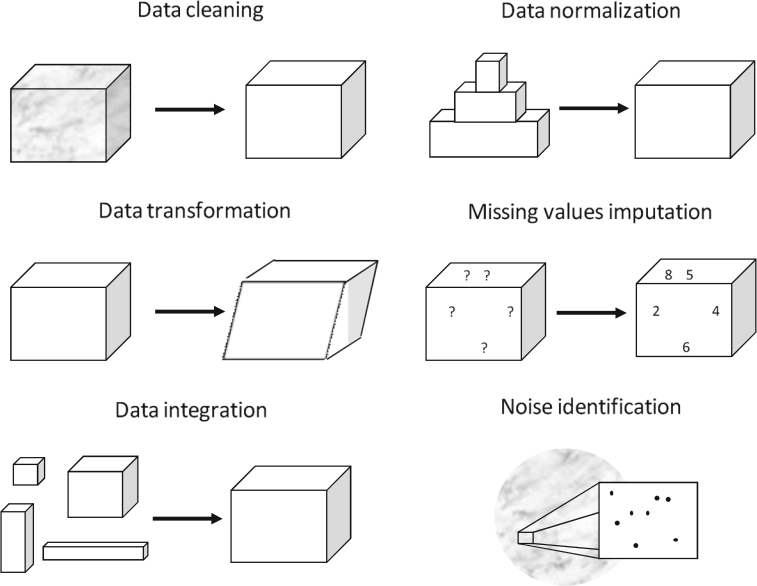
\includegraphics[width=.7\linewidth]{../img/data_preproc.png}}
    \normalcolor\caption{"`Preprocessing Tasks"' aus \cite[Seite 4]{garcia2016big}}
\end{figure}

Die folgenden Unterabschnitte erklären die Vorverarbeitungsschritte für die BfArM-Daten und beziehen sich damit auf die in \ref{abweichungen} genannten Abweichungen. Die Schritte erfolgen in der gelisteten Reihenfolge. Obwohl die Daten nach dem CSV-Parsing schon in einer von der Programmiersprache abhängigen Struktur vorliegen, wird zur Erklärung trotzdem noch die Datei-Struktur verwendet.

\subsection{Datennormalisierung}

\newpara{6-Spalten-Umsteiger}

Sowohl die ICD-10-GM Versionen 2004 und 2.0, als auch die OPS Version 2.1 beinhalteten Umsteiger in folgendem Format:

\codeBoxLD{A00.0;A00.0;A;A;0;UNDEF}{1-202;1-202;A;A;;}

Um diese an das ICD-10-GM Format von 2024 anzupassen, werden die letzten beiden Spalten entfernt. 

\newpara{OPS Umsteiger}

Für OPS Versionen ab 2010 sehen die Umsteiger-Einträge so aus:

\codeBoxL{1-100;N;1-100;N;A;A}

Durch Entfernung der zweiten und vierten Spalte stimmen diese mit den ICD-10-GM Umsteiger Format von 2024 überein. 

\newpara{OPS 6-Spalten-Umsteiger, altes Format}

Die OPS Versionen 2009 bis 2006 hatten ebenfalls sechs Spalten für die Umsteiger, aber in einer anderen Reihenfolge:

\codeBoxL{1-100;1-100;N;N;A;A}

Hier müssen also die dritte und vierte Spalte entfernt werden. 

\newpara{OPS 5-Spalten-Umsteiger}

Die Umsteiger von OPS Version 2005 waren in einem ganz eigenen Format geschrieben:

\codeBoxL{5-062.0;5-062.0;N;A;A\newline
5-062.1;5-062.1;N;A;A\newline
5-062.2;5-062.8;J;E;E\newline
5-062.3;5-062.8;J;B;B}

Hier wird dritte Spalte entfernt und außerdem werden die Sonderformen für automatische Überleitbarkeit von \texttt{B} und \texttt{E} nach \texttt{A} umbenannt. 

\subsection{Imputation}

Für Umsteiger der OPS Version 2.0 gibt es nur drei Spalten: 

\codeBoxLD{1-208.0;A;1-209.0}{1-208.x;;1-209.4}

Die zweite Spalte zeigt allein die Überleitbarkeit an. Für die Angleichung an das ICD-10-GM Format von 2024 wird also die zweite Spalte entfernt und gedoppelt angehängt. Aus den beiden Beispielzeilen wird damit:

\codeBoxLD{1-208.0;1-209.0;A;A}{1-208.x;1-209.4;;}

\subsection{Datenbereinigung}

\newpara{KOMBI-Kode} Aus OPS Versionen 2.1 und 2.0 wird die erste Zeile der Kode-Datei entfernt, welche den KOMBI-Eintrag enthält. 

\newpara{None statt UNDEF} Für OPS Versionen 2009 bis 2004 wird der Kode-Wert \texttt{None} durch \texttt{UNDEF} ersetzt, sowohl in den Kodes-, als auch in den Umsteiger-Dateien. 

\newpara{Kreuz-Stern-System} Für die ICD-10-GM Versionen 2.0 und 1.3 werden die Zeichen \texttt{+}, \texttt{*} und \texttt{!} aus den Kode-Werten entfernt -- sowohl in der Kodes-, als auch der Umsteiger-Datei.

\newpara{Punkt-Strich-Notation} Für die ICD-10-GM Versionen 2004, 2.0 und 1.3 wird zuerst die Zeichenfolge \texttt{.-} aus den Kode-Werten in beiden Dateitypen entfernt. Danach wird nochmals \texttt{-} entfernt. Die Reihenfolge ist wichtig, weil in Version 2004 zum Beispiel Kodes \texttt{A00.-} und \texttt{G82.1-} vorkommen. 

\subsection{Instanzreduktion}
 
\newpara{Umsteiger}

Für viele Versionen sind über 90\% der Umsteiger-Einträge automatische Überleitungen in den gleichen Kode. Diese müssen also gar nicht in eine Applikation aufgenommen werden, unter der Annahme, dass nicht vorhandene Umsteiger gleich automatische Überleitungen sind. In dem Fall können alle Umsteiger ausgeschlossen werden, bei denen der neue Kode gleich dem alten Kode ist und die automatische Überleitbarkeit in beide Richtungen gegeben ist. 

\newpara{Nicht-endständige Umsteiger}

Die Überleitung von ICD-10-GM Version 2.0 auf 1.3 ist der einzige Fall, in dem die Umsteiger-Datei nicht-endständige Kodes enthält. Durch das Entfernen der Sonderzeichen von Punkt-Strich-Notation und Kreuz-Stern-System gibt es außerdem doppelte Einträge in der ersten Spalte, das heißt bei den Kodes der Vorgänger-Version. Folgende Funktion\footnote{Der Pseudocode ist beschrieben in Struktogrammen nach \cite{nassishneid}. Die später vorkommenden Algorithmen zur Umsteiger-Suche enthalten viele Variablenzuweisungen, die abhängig von einer Bedingung sind und deren parallele Darstellung in Nassi-Shneidermann-Diagrammen übersichtlicher ist. Sie werden also im Sinne der Einheitlichkeit ebenfalls für den Algorithmus in diesem Abschnitt verwendet.}
entfernt die überflüssigen Einträge.

Angenommen die Kodes befinden sich in einem Array mit Index von 0 bis (n-1), zum Beispiel für die ersten sechs Zeilen der Umsteiger-Datei aus ICD-10-GM, Überleitung 2.0 nach 1.3: 

\begingroup
\renewcommand{\arraystretch}{1.2}
\setlength{\tabcolsep}{12pt}
\begin{tabular}{cll}
Index & old (Alter Kode) & new (Neuer Kode) \\
\hline
0 & \texttt{A00} & \texttt{A00.0}  \\
1 & \texttt{A00} & \texttt{A00.1} \\
2 & \texttt{A00} & \texttt{A00.9} \\
3 & \texttt{A00.0} & \texttt{A00.0} \\
4 & \texttt{A00.1} & \texttt{A00.1} \\
5 & \texttt{A00.9} & \texttt{A00.9} \\
\end{tabular}
\endgroup

\newpara{RemoveNonTerminal}

Funktionsparameter:

\begin{itemize}
\item \texttt{\$data} \newline Umsteiger-Einträge
\end{itemize}

Lokale Variablen:

\begin{itemize}
\item \texttt{\$index}
  \newline Der Umsteiger-Eintrag, der aktuell verarbeitet wird.
  \newline Die Funktion läuft vom letztem Eintrag zum ersten.
\item \texttt{\$current}
  \newline Der alte Kode des aktuellen Umsteiger-Eintrags.
  \newline Hierbei bedeutet \$data[ \$index ][ 'old' ] Zugriff auf Zeile mit Index = Wert von \$index und Spalte 'Alter Kode'. Zum Beispiel: data[ 4 ][ 'old' ] = \texttt{A00.1}.
\item \texttt{\$prev}
  \newline Der alte Kode des zuletzt verarbeiteten Umsteiger-Eintrags.
  \newline Die Variable wird auf \$current gesetzt, wenn der Eintrag \emph{nicht} entfernt wird.
\end{itemize}

Anmerkungen:

\begin{itemize}
\item Die IF-Bedingung bezieht sich auf String-basierte Operationen; also contains: "`enthält"' als Sub-String und length: Anzahl der Zeichen im String.
\item remove: Entfernt eine ganze Zeile. 
\end{itemize}

\begin{centernss}
\small
\begin{struktogramm}(120,84)
    \assign[\heightNS]{\$index = count(\$data) - 1}
    \assign[\heightNS]{\$current = \$data[ \$index ][ 'old' ]}
    \while[\heightNS]{WHILE \$index > 0}
    \assign[\heightNS]{\$prev = \$data[ \$index-1 ][ 'old' ]}
    \ifthenelse[24]{2}{2}{IF \$current contains \$prev AND length(\$current) > length(\$prev)}{Y}{N}
        \assign[\heightNS]{remove \$data[ \$index-1 ]}
    \change
        \assign[\heightNS]{\$current = \$prev}
    \ifend
    \assign[\heightNS]{\$index = \$index - 1}
    \whileend
    \assign[\heightNS]{re-index \$data}
\end{struktogramm}
\end{centernss}

Beispiel-Array nach Durchlaufen des Algorithmus:

\begingroup
\renewcommand{\arraystretch}{1.2}
\setlength{\tabcolsep}{12pt}
\begin{tabular}{cll}
Index & old (Alter Kode) & new (Neuer Kode) \\
\hline
0 & \texttt{A00.0} & \texttt{A00.0} \\
1 & \texttt{A00.1} & \texttt{A00.1} \\
2 & \texttt{A00.9} & \texttt{A00.9} \\
\end{tabular}
\endgroup

\newpara{Nicht-endständige Kodes}

Für die meisten Anwendungen sind eigentlich nur die endständigen Kodes relevant. Statt diese bei jeder Operation herauszufiltern, können beim einmaligen Einlesen der Daten auch einfach die nicht-endständigen Kodes ausgeschlossen werden. Zu diesem Zweck funktioniert der oben erklärte Algorithmus ebenfalls. 

\subsection{Integration zusätzlicher Informationen}

Im nächsten Abschnitt wird erklärt, wie ermittelt wird, ob es zu einem Kode einer bestimmten Version Umsteiger in einer älteren oder neueren Version gibt. Um diese zusätzliche Information speichern zu können, werden die Kodes um eine Spalte erweitert.
